\documentclass[11pt,english,onehalfspacing,headsepline]{MastersDoctoralThesis}

\usepackage[utf8]{inputenc} % Required for inputting international characters
\usepackage[T1]{fontenc} % Output font encoding for international characters

\usepackage{amsmath}
\usepackage{amsthm}
\usepackage{amssymb}
\usepackage{mathtools}
\usepackage{tikz}
\usepackage{setspace}
\usepackage{extarrows}
\usepackage{listings}
\usepackage{makeidx}
\usepackage{float}

\lstset{
  basicstyle=\footnotesize,        % the size of the fonts that are used for the code
  breaklines=true,                 % sets automatic line breaking
  captionpos=b,                    % sets the caption-position to bottom
  frame=single,	                   % adds a frame around the code
  keepspaces=true,                 % keeps spaces in text, useful for keeping indentation of code (possibly needs columns=flexible)
  numbers=left,                    % where to put the line-numbers; possible values are (none, left, right)
  numbersep=10pt,                   % how far the line-numbers are from the code
  numberstyle=\tiny,
  tabsize=4,	                   % sets default tabsize to 2 spaces
  title=\lstname,           % show the filename of files included with \lstinputlisting; also try caption instead of title
}

\newcommand{\supp}{\mathrm{supp}}
\newcommand{\sus}{\mathrm{sus}}
\newcommand{\im}{\mathrm{Im}}

\usetikzlibrary{arrows,chains,matrix,positioning,scopes}
\makeatletter
\tikzset{join/.code=\tikzset{after node path={%
\ifx\tikzchainprevious\pgfutil@empty\else(\tikzchainprevious)%
edge[every join]#1(\tikzchaincurrent)\fi}}}
\makeatother

\tikzset{>=stealth',every on chain/.append style={join},
         every join/.style={->}}
\tikzstyle{labeled}=[execute at begin node=$\scriptstyle,
   execute at end node=$]

\newtheorem{defi}{Definition}[section]
\newtheorem{lem}{Lemma}[section]
\newtheorem{conj}{Conjecture}[section]
\newtheorem{rem}{Remark}[section]
\newtheorem{prop}{Proposition}[section]
\newtheorem{thm}{Theorem}[section]
\newtheorem{cor}{Corollary}[section]
\newtheorem{expl}{Example}[section]
\usepackage{mathpazo} % Use the Palatino font by default

%\usepackage[backend=bibtex,style=authoryear,natbib=true]{biblatex} % Use the bibtex backend with the authoryear citation style (which resembles APA)

%\addbibresource{example.bib} % The filename of the bibliography

%\usepackage[autostyle=true]{csquotes} % Required to generate language-dependent quotes in the bibliography

\usepackage[ngerman]{datetime}

\newdateformat{myformat}{\THEDAY{. }\monthnamengerman[\THEMONTH] \THEYEAR}

%----------------------------------------------------------------------------------------
%	MARGIN SETTINGS
%----------------------------------------------------------------------------------------

\geometry{
	paper=a4paper, % Change to letterpaper for US letter
	inner=2.5cm, % Inner margin
	outer=3.8cm, % Outer margin
	bindingoffset=.5cm, % Binding offset
	top=1.5cm, % Top margin
	bottom=1.5cm, % Bottom margin
	%showframe, % Uncomment to show how the type block is set on the page
}

%----------------------------------------------------------------------------------------
%	THESIS INFORMATION
%----------------------------------------------------------------------------------------

\thesistitle{Cosystoles and Cheeger Constants\\of the Simplex} % Your thesis title, this is used in the title and abstract, print it elsewhere with \ttitle
\supervisor{Prof. Dr. Dmitry \textsc{Feichtner-Kozlov}} % Your supervisor's name, this is used in the title page, print it elsewhere with \supname
\examiner{} % Your examiner's name, this is not currently used anywhere in the template, print it elsewhere with \examname
\degree{Doktor der Naturwissenschaften (Dr. rer. nat.)} % Your degree name, this is used in the title page and abstract, print it elsewhere with \degreename
\author{Kai Michael \textsc{Renken}} % Your name, this is used in the title page and abstract, print it elsewhere with \authorname
\addresses{} % Your address, this is not currently used anywhere in the template, print it elsewhere with \addressname

\subject{Mathematics} % Your subject area, this is not currently used anywhere in the template, print it elsewhere with \subjectname
\keywords{} % Keywords for your thesis, this is not currently used anywhere in the template, print it elsewhere with \keywordnames
\university{\href{http://www.uni-bremen.de}{Universität Bremen}} % Your university's name and URL, this is used in the title page and abstract, print it elsewhere with \univname
\department{\href{http://alta.uni-bremen.de}{ALTA - Institute for Algebra, Geometry, Topology and their Applications}} % Your department's name and URL, this is used in the title page and abstract, print it elsewhere with \deptname
\group{{Fachbereich 3}} % Your research group's name and URL, this is used in the title page, print it elsewhere with \groupname
\faculty{\href{http://fb3.uni-bremen.de}{Fachbereich 3 - Mathematik und Informatik}} % Your faculty's name and URL, this is used in the title page and abstract, print it elsewhere with \facname

\AtBeginDocument{
\hypersetup{pdftitle=\ttitle} % Set the PDF's title to your title
\hypersetup{pdfauthor=\authorname} % Set the PDF's author to your name
\hypersetup{pdfkeywords=\keywordnames} % Set the PDF's keywords to your keywords
}

\makeindex

\begin{document}

\frontmatter % Use roman page numbering style (i, ii, iii, iv...) for the pre-content pages

\pagestyle{plain} % Default to the plain heading style until the thesis style is called for the body content

%----------------------------------------------------------------------------------------
%	TITLE PAGE
%----------------------------------------------------------------------------------------

\begin{titlepage}
\begin{center}


\includegraphics[scale=0.3]{Logo.jpg} % University/department logo - uncomment to place it

\textsc{\Large Dissertation}\\[0.5cm] % Thesis type

\HRule \\[0.4cm] % Horizontal line
{\huge \bfseries \ttitle\par}\vspace{0.4cm} % Thesis title
\HRule \\[1.5cm] % Horizontal line
 
\begin{minipage}[t]{0.4\textwidth}
\begin{flushleft} \large
\emph{Autor:}\\
{\authorname} % Author name - remove the \href bracket to remove the link
\end{flushleft}
\end{minipage}
\begin{minipage}[t]{0.4\textwidth}
\begin{flushright} \large
\emph{Betreuer:} \\
{\supname} % Supervisor name - remove the \href bracket to remove the link  
\end{flushright}
\end{minipage}\\[3cm]
 
\vfill

\large \textit{Dissertation zur Erlangung des akademischen Grades \\ \degreename}\\[0.3cm] % University requirement text
\textit{}\\[0.4cm]
\facname\\[2cm] % Research group name and department name
 
\vfill

{\large \myformat\today}\\[4cm] % Date
 
\vfill
\end{center}
\end{titlepage}

%----------------------------------------------------------------------------------------
%	ZUSAMMENFASSUNG
%----------------------------------------------------------------------------------------

\begin{Zusammenfassung}
Das zentrale Thema dieser Arbeit ist, Methoden zu entwickeln, um die kosystolische Norm und die Korandausdehnung einer Kokette bestimmen oder zumindest besser abschätzen zu können. Diese Werte sind die Grundlage für die Bestimmung der Cheeger-Konstanten eines simplizialen Komplexes. Wir entwickeln einige strukturtheoretische Aussagen zur kosystolischen Norm von Koketten, in der wir unter anderem eine interessante Verbindung zwischen jener Norm und der Hitting-Zahl eines bestimmten Mengensystems untersuchen (Kapitel \ref{Chapter2}). In Kapitel \ref{Chapter3} schränken wir unsere Untersuchungen auf eindimensionale Kosystolen eines Simplexes ein, welche ein wenig einfacher zu verstehen sind, sodass wir in diesem Fall oft bessere Resultate liefern können, unter anderem die explizite Bestimmung der größten eindimensionalen Kosystolen eines Simplexes und eine ungefähre Übersicht, wie alle \(1\)-Kosystolen eines Simplexes im sogenannten kosystolischen Komplex angeordnet sind. Außerdem beweisen wir die Ungleichung \(h_1(\Delta^{[n]})>\frac{n}{3}\) für den Fall \(n=16\), was uns in der Vermutung bestärkt, dass diese Ungleichung allgemein gilt, falls \(n\) eine Zweierpotenz ist. In Kapitel \ref{Chapter6} untersuchen wir einige alternative Verallgemeinerungen der klassischen Cheeger-Konstante, mit denen man einfacher arbeiten könnte und zeigen, dass diese verschiedenen Konstanten auf einer großen Familie von simplizialen Komplexen gleich sind. In Kapitel \ref{Chapter4} lösen wir ein schönes kombinatorisches Anordnungsproblem, welches nicht in direktem Zusammenhang mit dem Rest dieser Arbeit steht, aber während grundlegener Überlegungen darüber aufkam und interessant genug sein sollte, dem Leser ebenso zur Verfügung gestellt zu werden. In Anhang \ref{AppendixB} geben wir einen Algorithmus zur konkreten Berechnung der Lösungen des Anordnungsproblems aus Kapitel \ref{Chapter4} an.
\end{Zusammenfassung}

%----------------------------------------------------------------------------------------
%	ABSTRACT PAGE
%----------------------------------------------------------------------------------------

\begin{abstract}
%\addchaptertocentry{\abstractname} % Add the abstract to the table of contents
The central interest of this thesis is to develop tools to get hands on the cosystolic norm and the coboundary expansion of a cochain, values which are important to determine the Cheeger constants of a simplicial complex. We develop some structural theory about the cosystolic norm of a cochain, in which we, among other small results, study an interesting connection between that norm and the hitting number of a certain set system (see Chapter \ref{Chapter2}). In Chapter \ref{Chapter3} we restrict our research to \(1\)-dimensional cosystoles of a simplex which are slightly easier to understand, so we can provide more explicit results for that case, including the explicit determination of the largest \(1\)-dimensional cosystoles of a simplex and a rough insight, how all \(1\)-cosystoles of a simplex in a certain dimension can be arranged in the so-called cosystolic complex. Furthermore, we prove the strict inequality \(h_1(\Delta^{[n]})>\frac{n}{3}\) for the case \(n=16\), which strengthens our conjecture that this strict inequality holds in general if \(n\) is a power of \(2\). In Chapter \ref{Chapter6} we study some alternative ways to generalize the classical Cheeger constant which might be easier to access and prove that these different constants equal for a large family of simplicial complexes. In Chapter \ref{Chapter4} we solve a beautiful combinatorial ordering problem, which is not directly related to the main subject of this thesis but arose during considerations about that and should be worth to be provided to the reader as well. In Appendix \ref{AppendixB} we give an algorithm for the exact calculation of the solutions of the ordering problem from Chapter \ref{Chapter4}.
\end{abstract}

%----------------------------------------------------------------------------------------
%	ACKNOWLEDGEMENTS
%----------------------------------------------------------------------------------------

\begin{acknowledgements}
I want to thank my family, who always encouraged me on my academic way and especially my mother Angela Schneider who always found the right cheering as well as hard words, that helped me through all the hard times that arose on this way. I also want to thank my project advisor Prof. Dr. Dmitry Feichtner-Kozlov, who introduced me to the beautiful subject of Cheeger constants as well as all my colleages at the University of Bremen who brightened every day at the office with enlightening discussions and a warm, welcoming athmosphere. Espacially, I thank Fabian Redecker, who has been a reliable companion through my whole academic and private life. And at the end, very special thanks to Hannah Söger for her love and support at all times.
\end{acknowledgements}

%----------------------------------------------------------------------------------------
%	LIST OF CONTENTS/FIGURES/TABLES PAGES
%----------------------------------------------------------------------------------------

\tableofcontents % Prints the main table of contents

%----------------------------------------------------------------------------------------
%	DEDICATION
%----------------------------------------------------------------------------------------

%\dedicatory{Dedicated to my mother} 

%----------------------------------------------------------------------------------------
%	THESIS CONTENT - CHAPTERS
%----------------------------------------------------------------------------------------

\mainmatter % Begin numeric (1,2,3...) page numbering

\pagestyle{thesis} % Return the page headers back to the "thesis" style

% Include the chapters of the thesis as separate files from the Chapters folder
% Uncomment the lines as you write the chapters
%\pagenumbering{Roman}
% Preliminaries

\addcontentsline{toc}{chapter}{Preliminaries}
\manualmark
\markboth{Preliminaries}{Preliminaries}

\chapter*{Preliminaries}

\label{Preliminaries}

Let us shortly recall some basic algebraic and combinatorial concepts, which we will use within this thesis.

\section*{Simplicial Complexes}

\index{Simplicial complex}
Let \(S\) be some set (whose elements are called \textbf{vertices})\index{Vertex} and \(X\subseteq 2^S\) a family of subsets of \(S\) (we will use the notation \(2^S\) for the power set of \(S\) within the whole thesis), such that for all \(\sigma\in X\) and all \(\sigma'\subseteq\sigma\) we have \(\sigma'\in X\). Then we call \(X\) an \textbf{(abstract) simplicial complex}. We just use the notation "simplicial complex" in this thesis, because we will only consider abstract simplicial complexes and are not interested in their geometric realization.\\
\\
An element of cardinality \(k+1\) of a simplicial complex \(X\) is called \(k\)-\textbf{simplex} \index{Simplex} and a \textbf{face}\index{Face} of a \(k\)-simplex \(\sigma\in X\) is a (\(k-1\))-simplex \(\sigma'\in X\), such that \(\sigma'\subset\sigma\). Furthermore, we denote the \(k\)-\textbf{skeleton} \index{Skeleton} of a simplicial complex \(X\) by
\[
X(k)\coloneqq \left\{\sigma\in X\;\text{:}\;\left|\sigma\right|\leq k+1\right\},
\]
and the \textbf{uniform} \(k\)-\textbf{skeleton} of \(X\) by
\[
X^{(k)}\coloneqq \left\{\sigma\in X\;\text{:}\;\left|\sigma\right|=k+1\right\}
\]
\\
Let \(\sigma\subset S\) be a simplex and \(s\in S\setminus\sigma\), then the simplex constructed by "adding" \(s\) to \(\sigma\) is denoted by \((\sigma,s)\coloneqq \sigma\cup\left\{s\right\}\).\\
For a simplicial complex \(X\) and a simplex \(\sigma\in X\) we call \(\dim(\sigma)\coloneqq |\sigma|-1\) the \textbf{dimension}\index{Dimension} of \(\sigma\) and \(\dim(X)\coloneqq \max\left\{\dim(\sigma):\sigma\in X\right\}\) the \textbf{dimension} of \(X\) (if it exists). Furthermore, for simplices \(\sigma\) and \(\sigma'\), such that \(\sigma'\subseteq\sigma\) the \textbf{codimension}\index{Codimension} of \(\sigma'\) in \(\sigma\) is defined as \(\dim(\sigma)-\dim(\sigma')\). 
\\
A simplicial complex is called \textbf{finite} if its vertex set is finite and \textbf{finite dimensional} if its dimension is finite.\\
The most frequently considered simplicial complex in this thesis will be the complex induced by the standard simplex on \(n\) vertices. It can be considered as the complete power set of \([n]\coloneqq\left\{i\in\mathbb{N}:1\leq i\leq n\right\}\) and we will denote it by \(\Delta^{[n]}\coloneqq 2^{[n]}\).

\section*{Co- / Chain Complexes \& Co- / Homology}

Let \(X\) be a simplicial complex, then
\[
C_k(X,\mathbb{Z}_2)\coloneqq \left\{\sum\limits_{i\in I}c_i\sigma_i\::\:\sigma_i\in X^{(k)}\text{, }c_i\in\mathbb{Z}_2\right\}
\]
is called the \(k\)-th \textbf{chain group}\index{Chain} of \(X\), where \(I\) is some index set. (The elements of \(C_k(X,\mathbb{Z}_2)\) are called \(k\)-\textbf{chains})\\
Note, that in general we have more possible coefficient systems than \(\mathbb{Z}_2\) and \(X\) can be any topological space, but we will restrict ourselves to simplicial complexes in this thesis. Furthermore, since we only consider chain groups with \(\mathbb{Z}_2\)-coefficients in this thesis, we will use the notation \(C_k(X)\coloneqq C_k(X,\mathbb{Z}_2)\).\\
The linear map \(\partial_k:C_{k+1}(X)\rightarrow C_k(X)\) defined on a simplex \(\sigma=(v_0,\ldots,v_{k+1})\in X\) as
\[
\partial_k(\sigma)\coloneqq \sum\limits_{i=0}^{k+1}(-1)^i(v_0,\ldots,v_{i-1},v_{i+1},\ldots,v_{k+1})
\]
is called the \(k\)-th \textbf{boundary map}.\index{Boundary} Note, that the boundary maps have the property \(\partial_{k-1}\circ\partial_k=0\), so we always have \(\im(\partial_k)\subseteq\ker(\partial_{k-1})\).\\
\\
The \(k\)-th \textbf{homology group}\index{Homology} of \(X\) is defined as
\[
H_k(X)\coloneqq \frac{\ker(\partial_{k-1})}{\im(\partial_k)},
\]
where the elements in \(\ker(\partial_{k-1})\) are called k-\textbf{cycles}\index{Cycle} and the elements in \(\im(\partial_k)\) are called k-\textbf{boundaries}.\\
Dualizing this concept, we get the \(k\)-th \textbf{cochain group}\index{Cochain} of \(X\) by
\[
C^k(X)\coloneqq C^k(X,\mathbb{Z}_2)\coloneqq \left\{\varphi:C_k(X)\rightarrow\mathbb{Z}_2:\varphi\text{ is a linear map}\right\},
\]
whose elements are called \(k\)-\textbf{cochains}, the \(k\)-th \textbf{coboundary map}\index{Coboundary} \\
\(\delta^k:C^k(X)\rightarrow C^{k+1}(X)\) by \(\delta^k(\varphi)\coloneqq \varphi\circ\partial_k\), and the \(k\)-th \textbf{cohomology group}\index{Cohomology} of \(X\) by
\[
H^k(X)\coloneqq \frac{\ker(\delta^k)}{\im(\delta^{k-1})}
\]
Note, that \(\delta^k\circ\delta^{k-1}=0\) holds again which implies that we have \(\im(\delta^{k-1})\subseteq\ker(\delta^k)\).\\
Furthermore, the sequence
\[
\cdots\xlongrightarrow{\partial_{k+1}} C_{k+1}(X)\xlongrightarrow{\partial_k} C_k(X)\xlongrightarrow{\partial_{k-1}} C_{k-1}(X)\xlongrightarrow{\partial_{k-2}}\cdots\xlongrightarrow{\partial_0} C_0(X)\xlongrightarrow{\partial_{-1}}\left\{0\right\}
\]
is called a \textbf{chain complex}\index{Chain complex} and
\[
\left\{0\right\}\xlongrightarrow{\delta^{-1}}C^0(X)\xlongrightarrow{\delta^0}\cdots\xlongrightarrow{\delta^{k-2}} C^{k-1}(X)\xlongrightarrow{\delta^{k-1}} C^k(X)\xlongrightarrow{\delta^k} C^{k+1}(X)\xlongrightarrow{\delta^{k+1}}\cdots
\]
is called a \textbf{cochain complex}\index{Cochain complex}.\\
\\
Let us still introduce the concept of reduced homology / cohomology. If we consider the augmented chain complex
\[
\cdots\xlongrightarrow{\partial_{k+1}} C_{k+1}(X)\xlongrightarrow{\partial_k} C_k(X)\xlongrightarrow{\partial_{k-1}} C_{k-1}(X)\xlongrightarrow{\partial_{k-2}}\cdots\xlongrightarrow{\partial_0} C_0(X)\xlongrightarrow{\varepsilon}\mathbb{Z}_2\longrightarrow \left\{0\right\},
\]
with \(\varepsilon\left(\sum\limits_{i\in I}c_i\sigma_i\right)\coloneqq \sum\limits_{i\in I}c_i\) instead of the ordinary chain complex, then we call the corresponding homology groups the \textbf{reduced homology groups}\index{Reduced homology} of \(X\) and denote them by \(\tilde{H}_k(X)\). Note, that only the \(0\)-th reduced homology group differs from the ordinary \(0\)-th homology group, such that we have \(H_0(X)\cong\tilde{H}_0(X)\oplus\mathbb{Z}_2\) and \(H_k(X)\cong\tilde{H}_k(X)\) for all \(k\geq 1\). Dualizing this concept one can define reduced cohomology\index{Reduced cohomology} analogously.\\
\\
Since we are working with \(\mathbb{Z}_2\)-coeficients only, there is a very intuitive way to talk about chains (cochains, respectively). A \(k\)-chain is a linear combination of \(k\)-simplices with coefficients in \(\mathbb{Z}_2\), so it can just be considered as a subset of the uniform \(k\)-skeleton of the underlying simplicial complex \(X\). Furthermore, there is a one-to-one correspondence between chains and cochains, so to every chain \(c\in C_k(X)\) we can associate its characteristic cochain which we denote by \(c^*\in C^k(X)\) and for every cochain \(\varphi\in C^k(X)\) there exists a unique chain \(c\in C_k(X)\), such that we have \(c^*=\varphi\).\\
Let \(c\in C_k(X)\) be some chain and \(\varphi\in C^k(X)\) some cochain, then we denote the \textbf{evaluation}\index{Evaluation} of \(\varphi\) on \(c\) as
\[
\left\langle\varphi,c\right\rangle\coloneqq \varphi(c)\in\mathbb{Z}_2,
\]
and the \textbf{support}\index{Support} of \(\varphi\) as
\[
\supp(\varphi)\coloneqq \left\{\sigma\in X^{(k)}:\left\langle\varphi,\sigma\right\rangle=1\right\}
\]
Furthermore, we define the support of a chain \(c\in C_k(X)\) as \(\supp(c)\coloneqq \supp(c^*)\).\\
Even boundaries and coboundaries can be imagined very intuitively: The support of a boundary of a chain exactly consists of those simplices which are contained in an odd number of simplices from the support of the chain. The support of a coboundary exactly exists of those simplices which contain an odd number of simplices from the support of the cochain.\\
Note, that for simplicity we will omit natural inclusion maps of the type\\
\(i:\Delta^{[n]}\longrightarrow\Delta^{[n+d]}\) for some \(n,d\in\mathbb{N}\) when adding chains / cochains, so that for \(\varphi\in C^k(\Delta^{[n]})\text{, }\psi\in C^k(\Delta^{[n+d]})\) we will write \(\varphi+\psi\in C^k(\Delta^{[n+d]})\) instead of\\
\(i(\varphi)+\psi\in C^k(\Delta^{[n+d]})\). From the context it should always be clear what we mean.


\section*{Graphs \& Hypergraphs}

Let \(V\) be some set and \(E\subseteq\binom{V}{2}\) (we will always use the notation\\
\(\binom{V}{k}\coloneqq \left\{S\in 2^V:\left|S\right|=k\right\}\) to denote the set of all subsets of cardinality \(k\) of a set \(V\)). Then the pair \(G=\left(V,E\right)\) is called a \textbf{(simple) graph}\index{Graph}, where the elements of \(V\) are called \textbf{vertices}\index{Vertex} and the elements of \(E\) are called \textbf{edges}\index{Edge}. Since we only consider simple graphs (undirected graphs with no loops or double edges) in this thesis, we will just call them graphs. Even though we only consider undirected graphs, we want to stick to the common notation and denote an edge by \(e=(v,w)\) instead of using set brackets \(e=\{v,w\}\). In a graph \(G=(V,E)\) two vertices \(v_1,v_2\in V\) are called \textbf{adjacent}\index{Adjacent} if we have \((v_1,v_2)\in E\).\\
Note, that a graph can be considered as a \(1\)-dimensional simplicial complex, where \(V\) is the \(0\)-skeleton and \(E\) is the uniform \(1\)-skeleton.\\
According to the terminology of simplicial complexes we call a graph \textbf{finite}, if the number of vertices is finite.\\
A graph \(G=(V,E)\) is called \textbf{complete}, if \(E=\binom{V}{2}\) and a graph \(G'=(V',E')\) is called a \textbf{subgraph} of \(G=(V,E)\), if \(V'\subseteq V\) and \(E'\subseteq E\). Furthermore, we call a subgraph \(G'=(V',E')\) of \(G=(V,E)\) a \textbf{spanning subgraph}\index{Spanning subgraph} if \(E'\subseteq E\) and \(V'=V\). For every vertex \(v\in V\) of a graph \(G=(V,E)\) we call \(\deg_G(v)\coloneqq \left|\left\{w\in V:(v,w)\in E\right\}\right|\) the \textbf{degree}\index{Degree} of \(v\) and \(G\) is called \(t\)-\textbf{regular}\index{Regular graph} if we have \(\deg_G(v)=t\) for every \(v\in V\). Let \(S\subseteq V\) be a subset of vertices of a graph \(G=(V,E)\) then \(S\) is a \textbf{connected component}\index{Connected component} of \(G\) if for each pair of vertices \(v,v'\in S\) there exist vertices \(v_1,\ldots,v_k\in S\) such that \((v,v_1),(v_1,v_2),\ldots,(v_{k-1},v_k),(v_k,v')\in E\) and for each pair of vertices \(v\in S\) and \(w\in V\setminus S\) we have \((v,w)\notin E\). A graph is called \textbf{connected}\index{Connected} if it has only one connected compotent.\\
Two graphs \(G=(V,E)\) and \(G'=(V,E')\) are called \textbf{isomorphic}\index{Isomorphic}, if there exists a map \(f:V\rightarrow V\), such that \((i,j)\in E\) if and only if \((f(i),f(j))\in E'\). For a graph \(G=(V,E)\) the \textbf{isomorphism class}\index{Isomorphism class} of \(G\) is the set
\[
\left\{G'=(V,E'):G'\text{ and }G\text{ are isomorphic}\right\}
\]
A \textbf{hypergraph}\index{Hypergraph} is a pair \(H=(V,E)\), where the edge set \(E\subseteq 2^V\) can be any set of subsets of \(V\). Note, that every simplicial complex is a hypergraph, but not every hypergraph is a simplicial complex, since subsets of an edge do not have to be an edge in a hypergraph. If all edges of a hypergraph have the same cardinality \(k\), then we call it a \(k\)-\textbf{uniform hypergraph}. Analogously to the terminology of graphs, a hypergraph \(H'=(V',E')\) is called a \textbf{subhypergraph} of the hypergraph \(H=(V,E)\), if \(V'\subseteq V\) and \(E'\subseteq E\).

\automark[chapter]{chapter}
%\pagenumbering{arabic}
\setcounter{chapter}{0}
% Introduction

\chapter{Introduction}

\label{Introduction}
The classical Cheeger constant of a graph is a well-studied object and can be intuitively be imagined as a measure of connectivity of a graph, as follows: From a connected graph, we can delete edges to make it become disconnected, and so there exists a smallest (in terms of numbers of vertices) connected component. Now, the Cheeger constant is the smallest quotient that can appear by deviding the number of removed edges by the size of the smallest of the resulting connected components. So, formally the Cheeger constant of a graph \(G=(V,E)\) is then defined by:
\[
h(G):=\min\left\{\frac{|\delta(A)|}{|A|}\text{ : }A\subset V\text{, }1\leq |A|\leq\frac{|V|}{2}\right\},
\]
with \(\delta(A):=\left\{e=(v,w)\in E\text{ : }v\in A\text{, }w\in V\setminus A\right\}\).\\
\\
There is a lot of literature that studies this Cheeger constant for arbitrary graphs, whereas it is pretty easy to determine for the complete graph on \(n\)-vertices \(K_n\), where we have:
\[
h(K_n)=\left\lceil\frac{n}{2}\right\rceil
\]
In this thesis we want to investigate a higher-dimensional generalization of this Cheeger constant that was first introduced by Lineal and Meshulam (see \cite{2}) and later independently by Gromov (see \cite{3}) and is defined by the following construction:\\
\\
Let \(X\) be a simplicial complex and \(\varphi\in C^k(X)\), such that \(\|\delta^{k-1}(\phi)+\varphi\|\geq\|\varphi\|\) for every \(\phi\in C^{k-1}(X)\), where \(\delta^{k-1}\) denotes the coboundary map \(C^{k-1}(X)\rightarrow C^k(X)\), then we call \(\varphi\) a \(k\)-\textbf{cosystole}.\\
For general cochains \(\varphi\in C^k(X)\) we define the \textbf{cosystolic norm} of \(\varphi\) by:
\[
\|\varphi\|_{csy}:=\min\left\{\|\delta^{k-1}(\phi)+\varphi\|\text{ : }\phi\in C^{k-1}(X)\right\}
\]
Furthermore, any \(c\in C^k(X)\), satisfying \(c=\delta^{k-1}(\phi)+\varphi\) and \(\|c\|=\|\varphi\|_{csy}\) is called a \textbf{cosystolic form} of \(\varphi\).\\
\\
The quotient
\[
\|\varphi\|_{exp}:=\frac{\|\delta^k(\varphi)\|}{\|\varphi\|_{csy}}
\]
is called the \textbf{coboundary expansion} of \(\varphi\) and
\[
h_k(X):=\min\limits_{\varphi\in C^k(X)\text{, }\delta^k(\varphi)\neq 0}\|\varphi\|_{exp}
\]
is called the \(k\)-th \textbf{Cheeger constant} of \(X\).\\
\\
A cosystole \(\varphi\in C^k(X)\) is called a \textbf{Cheeger cosystole} if \(h_k(X)=\|\varphi\|_{exp}\).\\
\\
Note, that the classical Cheeger constant of a graph coincides with the \(0\)-th Cheeger constant \(h_0(X)\). For larger \(k\)'s the value of \(h_k(X)\) is not even known for all standard simplices \(X=\Delta^{[n]}\). By now we only have the estimate
\[
\frac{n}{k+2}\leq h_k(\Delta^{[n]})\leq\left\lceil\frac{n}{k+2}\right\rceil
\]
that was proven by Wallach and Meshulam (see \cite{4}), so we have the exact value \(h_k(\Delta^{[n]})=\frac{n}{k+2}\) when \(k+2\) devides \(n\). In \cite{1} Kozlov showed that the upper bound is archieved when \(k=n-3\), so we have \(h_{n-3}(\Delta^{[n]})=2\) and furthermore he showed that \(h_1(\Delta^{[n]})=\frac{n}{3}\) even holds for every \(n\) that is not a power of \(2\).\\
\\
In the first part of this thesis we will develop some theory about the cosystolic norm of cochains, since a better understanding of cosystoles seems to be the key knowledge to determine the Cheeger constants. In the second part we will focus on the special case of \(1\)-cosystoles and the first Cheeger constant, where we have an interesting graph theoretical approach introduced by Kozlov in \cite{1}, that seems to be suited well to investigate cosystoles in a combinatorial way.


% Chapter 2

\chapter{Detecting cosystoles}

\label{Chapter2}

When we want to determine whether a cochain is a cosystole or not until now we only have the original definition of cosystolicity, which does not seem to be very useful. In this chapter we want to develop tools to get hands on this problem and investigate the structure how cosystoles in certain simplicial complexes are arranged.

\section{Piercing sets and the cycle detection theorem}

The following definition is adopted from \cite{6}.

\begin{defi}
Let \(V\) be some set and \(\mathcal{F}\subseteq 2^V\) a family of finite subsets of \(V\). A subset \(P\subseteq V\) is called a \textbf{piercing set} of \(\mathcal{F}\) if we have \(P\cap F\neq\emptyset\) for all \(F\in\mathcal{F}\). The minimal cardinality of a piercing set of \(\mathcal{F}\), denoted by \(\tau(\mathcal{F})\), is called the \textbf{piercing number} of \(\mathcal{F}\).\\
For a \(v\in V\) and an \(F\in\mathcal{F}\) we say that \(F\) \textbf{is pierced by} \(v\), if \(v\in F\).
\end{defi}

\begin{expl}\label{example1}
Let \(V:=\left\{1,2,3,4,5\right\}\) and \(\mathcal{F}:=\left\{\{1,2\}\{2,3,4\},\{1,5\},\{2,4,5\}\right\}\), then we have \(\tau(\mathcal{F})=2\), since for example \(P:=\left\{2,5\right\}\) is a minimal piercing set of \(\mathcal{F}\).
\end{expl}

Later we will often talk about piercing numbers and piercing sets of families of \(k\)-chains, which we define as follows:

\begin{defi}
Let \(X\) be a simplicial complex and \(\mathcal{F}\subseteq C_k(X)\) a family of \(k\)-chains. The \textbf{piercing sets} and the \textbf{piercing number} of \(\mathcal{F}\) are defined as the piercing sets and the piercing number of the family \(\left\{supp(F)\text{ : }F\in\mathcal{F}\right\}\).
\end{defi}

In \cite{6} Kozlov stated the following useful method to bound the cosystolic norm of a cochain.

\begin{thm}[The cycle detection theorem]\label{theorem9}
Let \(X\) be a simplicial complex and \(\varphi\in C^k(X)\). Let now \(\mathcal{F}=\left\{\alpha_1,\ldots,\alpha_t\right\}\) be a family of \(k\)-cycles in \(C_k(X)\), such that \(\left\langle\varphi,\alpha_i\right\rangle=1\) for all \(1\leq i\leq t\), then we have:
\[
\|\varphi\|_{csy}\geq\tau(\mathcal{F})
\]
\begin{proof}
Let \(\psi\in C^{k-1}(X)\), then for any \(1\leq i\leq t\) we have:
\begin{align}
\langle\varphi+\delta^{k-1}(\psi),\alpha_i\rangle&=\langle\varphi,\alpha_i\rangle+\langle\delta^{k-1}(\psi),\alpha_i\rangle\notag\\
&=\langle\varphi,\alpha_i\rangle+\langle\psi,\partial_{k-1}(\alpha_i)\rangle\notag\\
&=\langle\varphi,\alpha_i\rangle+\langle\psi,0\rangle\notag\\
&=\langle\varphi,\alpha_i\rangle=1\notag
\end{align}
This means that we have \(supp(\varphi+\delta^{k-1}(\psi))\cap supp(\alpha_i)\neq\emptyset\) for all \(1\leq i\leq t\), so \(supp(\varphi+\delta^{k-1}(\psi))\) is a piercing set of \(\mathcal{F}\) and we get:
\[
\|\varphi+\delta^{k-1}(\psi)\|=|supp(\varphi+\delta^{k-1}(\psi))|\geq\tau(\mathcal{F})
\]
Since \(\psi\) was chosen arbitrarily we get the requested result.
\end{proof}
\end{thm}

The following corollary (a special case of the preceding theorem) was also stated by Kozlov in \cite{6}.

\begin{cor}
Let \(X\) be a simplicial complex and \(\varphi\in C^k(X)\).\\
Let now \(\mathcal{F}=\{\alpha_1,\ldots,\alpha_{\|\varphi\|}\}\) be a family of \(k\)-cycles in \(C_k(X)\), such that \(\left\langle\varphi,\alpha_i\right\rangle=1\) for all \(1\leq i\leq\|\varphi\|\) and \(supp(\alpha_i)\cap supp(\alpha_j)=\emptyset\) for all \(i\neq j\), then \(\varphi\) is a cosystole.
\begin{proof}
Since the supports of the cycles \(\alpha_1,\ldots,\alpha_{\|\varphi\|}\) are pairwise disjoint, we obviously have \(\tau(\mathcal{F})=\|\varphi\|\) and using the cycle detection theorem we are done.
\end{proof}
\end{cor}

\begin{expl}
Consider the cochain
\[
\varphi=\left(\{1,2,4\}+\{2,5,6\}+\{3,4,6\}+\{2,4,6\}\right)^*\in C^2(\Delta^{[6]})
\]
(Figure \ref{figure5:Figure 1} illustrates how the support of this cochain can be imagined) and the family of cycles
\begin{align*}
\mathcal{F}=\{&\{1,2,3\}+\{1,2,4\}+\{1,4,3\}+\{2,4,3\},\\
&\{1,2,5\}+\{1,2,6\}+\{1,5,6\}+\{2,5,6\},\\
&\{3,4,5\}+\{3,4,6\}+\{3,5,6\}+\{4,5,6\},\\
&\{1,3,5\}+\{1,3,6\}+\{1,4,5\}+\{1,4,6\}+\\
&\{2,3,5\}+\{2,3,6\}+\{2,4,5\}+\{2,4,6\}\}\subset C_2(\Delta^{[6]}).
\end{align*}
It is easy to check that we have \(\left\langle\varphi,\alpha\right\rangle=1\) for all \(\alpha\in\mathcal{F}\) and \(\tau(\mathcal{F})=4\), so we get \(\|\varphi\|_{csy}\geq 4\) by the cycle detection theorem. We can immediately see, that \(\varphi\) is a cosystole, either by the fact, that we always have \(\|\varphi\|_{csy}\leq \|\varphi\|\), so in our case we have \(\|\varphi\|=4=\|\varphi\|_{csy}\), or by using the preceding corollary, since the supports of the cycles in \(\mathcal{F}\) are pairwise disjoint.
\end{expl}

\begin{figure}[ht]
\centering
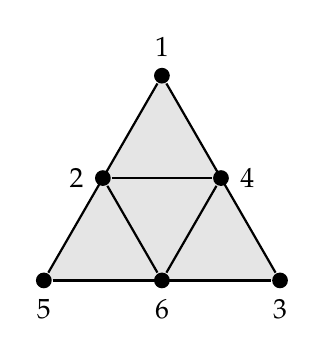
\begin{tikzpicture}[
       thick,
       acteur/.style={
         circle,
         fill=black,
         thick,
         inner sep=2pt,
         minimum size=0.2cm
       }
     ] 

	   \fill[fill=gray!20] (0,0)--(3,0)--(1.5,2.6);

       \node (a1) at (0,0) [acteur,label=below:5]{};
       \node (a2) at (3,0)[acteur,label=below:3]{}; 
       \node (a3) at (1.5,2.6) [acteur,label=above:1]{}; 
       \node (a4) at (0.75,1.3) [acteur,label=left:2]{}; 
       \node (a5) at (2.25,1.3) [acteur,label=right:4]{}; 
       \node (a6) at (1.5,0) [acteur,label=below:6]{};
  
       \draw (a1) -- (a2); 
       \draw (a2) -- (a3); 
       \draw (a1) -- (a3);
       
       \draw (a4) -- (a5);
       \draw (a5) -- (a6);
       \draw (a4) -- (a6);

\end{tikzpicture}
  \caption{The support of a $2$-cosystole (The gray triangles represent the four $2$-simplices)}
  \label{figure5:Figure 1}
\end{figure}


To get the best possible results using the cycle detection theorem, the challenge is now for a certain cochain \(\varphi\) to find families of cycles such that they have a large piercing number and \(\varphi\) evaluates to \(1\) on every cycle. The following construction seems to be suited well to get hands on this problem.\\
For a cochain \(\varphi\in C^k(X)\) we define the following set of cycles:
\[
\mathcal{T}_{\varphi}:=\left\{\partial_k(\sigma)\text{ : }\sigma\in supp(\delta^k(\varphi))\right\}
\]

\begin{prop}
Let \(\varphi\in C^k(X)\), then we have:
\[
\|\varphi\|_{csy}\geq\tau(\mathcal{T}_{\varphi})
\]
\begin{proof}
By the definition of the coboundary map, we obviously have\\
\(\left\langle\varphi,\partial_k(\sigma)\right\rangle=1\) for all \(\partial_k(\sigma)\in\mathcal{T}_{\varphi}\) and so by the cycle detection theorem we are done.
\end{proof}
\end{prop}

In many cases, even the equality \(\|\varphi\|_{csy}=\tau(\mathcal{T}_{\varphi})\) can be reached, but unfortunately this is not always true as the following example shows.

\begin{expl}
Let \(\varphi\in C^2(\Delta^{[6]})\) be the cosystole from Example \ref{example1}. We have:
\begin{align*}
\mathcal{T}_{\varphi}=\{&\{1,2,3\}+\{1,2,4\}+\{1,3,4\}+\{2,3,4\},\\
&\{1,2,4\}+\{1,2,5\}+\{1,4,5\}+\{2,4,5\},\\
&\{2,3,5\}+\{2,3,6\}+\{2,5,6\}+\{3,5,6\},\\
&\{1,2,5\}+\{1,2,6\}+\{1,5,6\}+\{2,5,6\},\\
&\{3,4,5\}+\{3,4,6\}+\{3,5,6\}+\{4,5,6\},\\
&\{1,3,4\}+\{1,3,6\}+\{1,4,6\}+\{3,4,6\}\}.
\end{align*}
It is easy to check that we get \(\tau(\mathcal{T}_{\varphi})=3\), but as shown in Example \ref{example1} we have \(\|\varphi\|_{csy}=4\).
\end{expl}

It seems to be very difficult to determine the piercing number of \(\mathcal{T}_{\varphi}\) explicitely, but the concept of piercing complexes might be useful on the way to solve this problem.

\section{Piercing complexes}

Let \(V\) be some set, \(\mathcal{F}\subset 2^V\) a family of subsets and \(P\) a piercing set of \(\mathcal{F}\). Then for any \(v\in V\) obviously \(P\cup\{v\}\) is also a piercing set of \(\mathcal{F}\). We can use this fact to construct a simplicial complex, which contains all information about the piercing sets for a given family of sets as follows:

\begin{defi}
Let \(V\) be a set and \(\mathcal{F}\subset 2^V\) a family of subsets. Then the \textbf{piercing complex} of \(\mathcal{F}\) is defined as:
\[
\Delta_{\mathcal{F}}:=\left\{V'\subseteq V,\text{ : }(V\setminus V')\cap F\neq\emptyset\text{ for all }F\in\mathcal{F}\right\}
\]
\end{defi}
So, \(\Delta_{\mathcal{F}}\) consists of all subsets of \(V\), such that their complements in \(V\) are piercing sets of \(\mathcal{F}\) and indeed, \(\Delta_{\mathcal{F}}\) defines a simplicial complex, since deleting an element from the complement of a piercing set is equivalent to adding an element to a piercing set, which preserves the condition of being a piercing set.\\

\begin{expl}
Let \(V\) be an arbitrary set and \(\mathcal{F}:=2^V\) its power set. Then the piercing complex \(\Delta_{\mathcal{F}}\) is empty, since even the complement of a single vertex \(v\in V\) is not a piercing set of \(\mathcal{F}\). More general for an arbitrary set \(V\) we have that \(\Delta_{\mathcal{F}}\) is empty if and only if \(\left\{v\right\}\in\mathcal{F}\), for all \(v\in V\).\\
On the other hand \(\Delta_{\mathcal{F}}\) is a complete simplex on \(\left|V\right|\) vertices if and only if \(\mathcal{F}\) is empty, since only in this case even the empty set is a piercing set of \(\mathcal{F}\).
\end{expl}

We can now reformulate the question of determining the piercing number \(\tau(\mathcal{F})\) by asking for the dimension of \(\Delta_{\mathcal{F}}\), since we have the equality:
\[
\tau(\mathcal{F})=\left| V\right|-dim(\Delta_{\mathcal{F}})-1
\]
Since our main interest in this section will be to investigate the piercing complex of \(\mathcal{T}_{\varphi}\) for a given cochain \(\varphi\in C^k(X)\) (where \(X\) is some simplicial complex) we will use a shorter notation for this piercing complex and set \(\Delta_{\varphi}:=\Delta_{\mathcal{T}_{\varphi}}\). Then the preceding formula turns to:
\[
\tau(\mathcal{T}_{\varphi})=|X^{(k)}|-dim(\Delta_{\varphi})-1
\]

% TO BE CHECKED !!!
%
%      |
%      |
%      v

%The first interesting observation about \(\Delta_{\varphi}\) is, that its top dimensional homology group vanishes in almost all cases.

%\begin{thm}
%Let \(n\geq k+3\) and \(\varphi\in C^k(X)\), then we have:
%\[
%H_{dim(\Delta_{\varphi})}(\Delta_{\varphi})\cong 0
%\]
%\begin{proof}
%Let \(\sigma\in\Delta_{\varphi}\) be a maximal simplex (i.e. for all \(v\in X^{(k)}\setminus\sigma\), we have \(\sigma\cup\{v\}\notin\Delta_{\varphi}\)). Then \(X^{(k)}\setminus\sigma\) is a minimal piercing set of \(\mathcal{T}_{\varphi}\) (i.e. for all \(v\in X^{(k)}\setminus\sigma\) we have that \(X^{(k)}\setminus (\sigma\cup\{v\})\) is not a piercing set of \(\mathcal{T}_{\varphi}\). Now, let \(v\in\sigma\) and \(w\in X^{(k)}\setminus\sigma\), such that \((\sigma\setminus\{v\})\cup\{w\}\in\Delta_{\varphi}\), and let
%\[
%P_w:=\left\{c\in\mathcal{T}_{\varphi}\text{ : }w\in c\text{, }w'\notin c\text{ for all }w'\in X^{(k)}\setminus\sigma\text{, }w'\neq w\right\}
%\]
%be the set of cycles from \(\mathcal{T}_{\varphi}\), that were pierced by \(w\) but by no other elements from \(X^{(k)}\setminus\sigma\). Then \(\{v\}\) must be a piercing set of \(P_w\) but since \(v\) and \(w\) are distinct, we get \(\left|P_w\right|=1\).
%\end{proof}
%\end{thm}

%      ^
%      |
%      |
%      
% TO BE CHECKED !!!

\begin{thm}
Let \(X\) be a simplicial complex and \(\varphi\in C^k(X)\), then we have:
\[
\tilde{H}_i(\Delta_{\varphi})\cong 0\quad\text{for all }i\leq k-1
\]
\begin{proof}
\begin{align*}
& \varphi\in C^k(X) \\
\Longrightarrow \quad & \text{For all }\sigma\in supp(\delta^k(\varphi))\text{ we have }\left|supp(\partial_k(\sigma))\right|=k+2 \\
\Longrightarrow \quad & \text{For all }S\subset X^{(k)}\text{ such that }\left|S\right|\leq k+1\text{ we have that } \\ & X^{(k)}\setminus S\text{ is a piercing set of }\mathcal{T}_{\varphi} \\
\Longrightarrow \quad & \Delta_{\varphi}\text{ has a full }k\text{-skeleton} \\
\Longrightarrow \quad & \tilde{H}_i(\Delta_{\varphi})\cong 0\text{ for all }i\leq k-1
\end{align*}
\end{proof}
\end{thm}

\begin{defi}
Let \(X\) be a simplicial complex on the vertex set \(V\). Then the simplicial complex
\[
X^{\lor}:=\left\{\sigma\subseteq V\text{ : }V\setminus\sigma\notin X\right\}
\]
is called the \textbf{Alexander dual} of \(X\).
\end{defi}

The following theorem can be found in \cite{8}.

\begin{thm}[The Alexander duality theorem]\label{theorem12}
Let \(X\) be a simplicial complex on \(n\) vertices and \(X^{\lor}\) its Alexander dual. Then we have:
\[
\tilde{H}_i(X)\cong\tilde{H}^{n-i-3}(X)
\]
\end{thm}

\begin{defi}
Let \(V\) be some set and \(\mathcal{F}\subseteq 2^V\) a family of subsets of \(V\). Then the simplicial complex
\[
\Delta\left[\mathcal{F}\right]:=\left\{\sigma\subseteq V\text{ : there exists an }F\in\mathcal{F}\text{ such that }\sigma\subseteq F\right\}
\]
is called the \textbf{induced complex} of \(\mathcal{F}\). 
\end{defi}

The following statement was developed in \cite{9}.

\begin{prop}\label{proposition13}
Let \(V\) be some set and \(\mathcal{F}\subseteq 2^V\) a family of subsets of \(V\). Then we have:
\[
\Delta\left[\bar{\mathcal{F}}\right]^{\lor}=\Delta_{\mathcal{F}}
\]
where we set \(\bar{\mathcal{F}}:=\left\{V\setminus F\text{ : }F\in\mathcal{F}\right\}\).
\begin{proof}
We have:
\begin{align*}
  & \sigma\in\Delta\left[\bar{\mathcal{F}}\right]^{\lor} \\
  \Longleftrightarrow \quad & V\setminus\sigma\notin\Delta\left[\bar{\mathcal{F}}\right] \\
  \Longleftrightarrow \quad & \nexists F\in\bar{\mathcal{F}}\text{ : }V\setminus\sigma\subseteq F \\
  \Longleftrightarrow \quad & \nexists F\in\bar{\mathcal{F}}\text{ : }(V\setminus\sigma)\cap(V\setminus F)=\emptyset \\
  \Longleftrightarrow \quad & \nexists F'\in\mathcal{F}\text{ : }(V\setminus\sigma)\cap F'=\emptyset \\
  \Longleftrightarrow \quad & V\setminus\sigma\text{ is a piercing set of }\mathcal{F} \\
  \Longleftrightarrow \quad & \sigma\in\Delta_{\mathcal{F}}
 \end{align*}
\end{proof}
\end{prop}

\begin{thm}
Let \(X\) be a finite simplicial complex and \(\varphi\in C^k(X)\), then we have:
\[
\tilde{H}_k(\Delta_{\varphi})\cong 0
\]
\begin{proof}
For all \(\partial_k(\sigma)\in\mathcal{T}_{\varphi}\) we have \(|supp(\partial_k(\sigma))|=k+2\), so we get:
\[
dim(\Delta[\bar{\mathcal{T}}_{\varphi}])=|X^{(k)}|-(k+2)-1=|X^{(k)}|-k-3
\]
Now, there exist no two simplices of dimension \(|X^{(k)}|-k-3\) in \(\Delta[\bar{\mathcal{T}}_{\varphi}]\),\\
such that they have a face in common, so we have:
\[
\tilde{H}_{|X^{(k)}|-k-3}(\Delta[\bar{\mathcal{T}}_{\varphi}])\cong 0
\]
By the Alexander duality theorem and Proposition \ref{proposition13} we get:
\[
\tilde{H}_k(\Delta_{\varphi})\cong\tilde{H}^k(\Delta_{\varphi})=\tilde{H}^{|X^{(k)}|-(|X^{(k)}|-k-3)-3}(\Delta_{\varphi})\cong 0,
\]
where the first isomorphy is true, because we consider homology / cohomology over a field and \(\Delta_{\varphi}\) is finite.
\end{proof}
\end{thm}

\section{Large cosystoles of a simplex}

In this section we focus our investigations onto the question, what is the largest norm, a cosystole can attain when the underlying simplicial complex is a complete simplex, where the first statement we make is still valid for general simplicial complexes. 

\begin{lem}\label{lemma10}
If \(k\) is odd, then we have:
\[
C_{max}(X,k)\geq\tau(\mathcal{T}_{\varphi}),
\]
with \(\varphi=\left(\sum\limits_{\sigma\in X^{(k)}}\sigma\right)^*\).
\begin{proof}
Since \(k\) is odd we have \(\langle\varphi,c\rangle=1\) for all \(c\in\mathcal{T}_{\varphi}\), so by the cycle detection theorem we get \(\|\varphi\|_{csy}\geq\tau(\mathcal{T}_{\varphi})\) and we are done.
\end{proof}
\end{lem}

A direct consequence of the preceding lemma is the following estimate. For simplicity we want to introduce the notation \(\mathcal{T}_n^k:=\mathcal{T}_{\varphi}\) for \(\varphi:=\left(\sum\limits_{\sigma\in\binom{[n]}{k+1}}\sigma\right)^*\).

\begin{prop}\label{proposition11}
Let \(k\) be odd, then we have:
\[
C_{max}(\Delta^{[n]},k)\geq \left\lceil\frac{\binom{n}{k+2}}{n-k-1}\right\rceil
\]
\begin{proof}
Obviously, we have \(|\mathcal{T}_n^k|=\binom{n}{k+2}\), so since any simplex \(\sigma\in\binom{[n]}{k+1}\) intersects the support of exactly \(n-k-1\) cycles from \(\mathcal{T}_n^k\), any piercing set of \(\mathcal{T}_n^k\) must contain at least \(\left\lceil\frac{\binom{n}{k+2}}{n-k-1}\right\rceil\) elements and by Lemma \ref{lemma10} we are done.
\end{proof}
\end{prop}

Using the preceding lemma we can determine a lower bound of the maximal size of the \(1\)-dimensional cosystoles in a simplex. A more elementary proof of this estimate is given as Proposition \ref{proposition3}) in the following chapter, where we will even see, that equality can be reached, shown in Theorem \ref{theorem1}.

\begin{thm}\label{theorem10}
\(C_{max}(\Delta^{[n]},1)\geq\binom{n}{2}-\left\lfloor\frac{n^2}{4}\right\rfloor\)
\begin{proof}
Asking for the smallest piercing set of \(\mathcal{T}_n^1\) is equivalent to asking for the largest triangle-free graph (i.e. a graph on \(n\) vertices, containing as many edges as posssible, but no complete graph on \(3\) vertices as a subgraph) and taking the complement. Mantel's theorem (see \cite{7}) says, that a triangle-free graph on \(n\) vertices has at most \(\left\lfloor\frac{n^2}{4}\right\rfloor\) edges, so we immediately get:
\[
\tau(\mathcal{T}_n^1)=\binom{n}{2}-\left\lfloor\frac{n^2}{4}\right\rfloor
\]
and by Lemma \ref{lemma10} we are done.
\end{proof}
\end{thm}

Unfortunately, determining the piercing number of \(\mathcal{T}_n^k\) for \(k\geq 2\), or equivalently, determining the largest \(k\)-uniform hypergraph on \(n\)-vertices, containing no complete \(k\)-uniform hypergraph on \(k+2\) vertices as a subhypergraph, seems to be very difficult (see \cite{7}), so we can not use the preceding procedure to say something about \(C_{max}(\Delta^{[n]},k)\) for larger \(k\)'s in general.\\
Eventhough, we can exactly determine this number for the ultimate and the penultimate proper dimension as follows.

\begin{thm}\label{theorem7}
\(C_{max}(\Delta^{[n]},n-2)=1\), for all \(n\geq 3\)
\begin{proof}
Let \(\sigma\in\binom{[n]}{n-1}\) be chosen arbitrarily, \(\varphi:=\sigma^*\in C^{n-2}(\Delta^{[n]})\) and\\
\(\mathcal{F}:=\left\{\alpha\right\}\), where \(\alpha\) is the boundary of the single (\(n-1\))-dimensional simplex in \(\Delta^{[n]}\). Obviously, we have \(\left\langle\varphi,\alpha\right\rangle=1\), since \(supp(\varphi)\cap supp(\alpha)=supp(\varphi)\) and \(\tau(\mathcal{F})=1\), so by the cycle detection theorem we have \(\|\varphi\|_{csy}\geq 1\).\\
Now, let \(\sigma_1,\sigma_2\in\binom{[n]}{n-1}\) be chosen arbitrarily again (\(\sigma_1\neq\sigma_2\)) and \(c:=\sigma_1\cap\sigma_2\). Then we have \(\delta^{n-3}(c^*)+\sigma_1^*+\sigma_2^*=0\), so there exists no (\(n-2\))-cosystole attaining norm \(2\) and we are done.
\end{proof}
\end{thm}

\begin{lem}\label{lemma12}
For \(n\geq 4\) we have:
\[
\tau(\mathcal{T}_n^{n-3})=\left\lceil\frac{n}{2}\right\rceil
\]
\begin{proof}
For each \(\sigma\in\binom{[n]}{n-2}\) there exist exactly two cycles \(\alpha_1,\alpha_2\in\mathcal{T}_n^{n-3}\)\\
(\(\alpha_1\neq\alpha_2\)), such that \(\sigma\in supp(\alpha_1)\cap supp(\alpha_2)\), so the largest possible number of cycles from \(\mathcal{T}_n^{n-3}\) that can be pierced by one simplex is two. Furthermore, we have \(\left|\mathcal{T}_n^{n-3}\right|=\binom{n}{n-1}=n\), so we get \(\tau(\mathcal{T}_n^{n-3})\geq\left\lceil\frac{n}{2}\right\rceil\).\\
On the other hand, for all \(\alpha_1,\alpha_2\in\mathcal{T}_n^{n-3}\) there exists a \(\sigma\in\binom{[n]}{n-2}\), such that\\
\(\sigma\in supp(\alpha_1)\cap supp(\alpha_2)\), so we get \(\tau(\mathcal{T}_n^{n-3})\leq\left\lceil\frac{n}{2}\right\rceil\).
\end{proof}
\end{lem}

\begin{lem}\label{lemma13}
Let \(S\subset\binom{[n]}{n-2}\), such that \(\left|S\right|\geq\left\lfloor\frac{n}{2}\right\rfloor+1\), then there exist \(\sigma,\sigma'\in S\) \((\sigma\neq\sigma')\), such that \(\left|\sigma\cap\sigma'\right|=n-3\).
\begin{proof}
For \(\sigma,\sigma'\in\binom{[n]}{n-2}\) the condition \(\left|\sigma\cap\sigma'\right|<n-3\) is equivalent to the condition \(([n]\setminus\sigma)\cap([n]\setminus\sigma')=\emptyset\). Since we obviously have \(\left|[n]\setminus\sigma\right|=2\) for all \(\sigma\in\binom{[n]}{n-2}\) we can find at most \(\left\lfloor\frac{n}{2}\right\rfloor\) simplices \(\sigma_1,\ldots,\sigma_{\left\lfloor\frac{n}{2}\right\rfloor}\in\binom{[n]}{n-2}\), such that the sets \([n]\setminus\sigma_1,\ldots,[n]\setminus\sigma_{\left\lfloor\frac{n}{2}\right\rfloor}\) are pairwise disjoint and we are done.
\end{proof}
\end{lem}

\begin{thm}
\(C_{max}(\Delta^{[n]},n-3)=\left\lfloor\frac{n}{2}\right\rfloor\), for all \(n\geq 4\)
\begin{proof}
Let \(S\subset\binom{[n]}{n-2}\) be a minimal piercing set of \(\mathcal{T}_n^{n-3}\) as constructed in the proof of Lemma \ref{lemma12} and \(\varphi:=S^*\in C^{n-3}(\Delta^{[n]})\).\\
If \(n\) is even, then \(n-3\) is odd, so using Lemma \ref{lemma10} and Lemma \ref{lemma12} we have:
\[
C_{max}(\Delta^{[n]},n-3)\geq\tau(\mathcal{T}_n^{n-3})=\frac{n}{2}
\]
If \(n\) is odd then by the construction of \(\varphi\) there exists exactly one \(\alpha'\in\mathcal{T}_n^{n-3}\), such that \(\left\langle\varphi,\alpha'\right\rangle=0\), since \(\left|supp(\alpha')\cap supp(\varphi)\right|=2\). Set \(\mathcal{F}:=\mathcal{T}_n^{n-3}\setminus\alpha'\), then we have \(\left\langle\varphi,\alpha\right\rangle=1\) for all \(\alpha\in\mathcal{F}\) and \(\tau(\mathcal{F})\geq\tau(\mathcal{T}_n^{n-3})-1=\left\lceil\frac{n}{2}\right\rceil-1=\left\lfloor\frac{n}{2}\right\rfloor\) by Lemma \ref{lemma12}, so by the cycle detection theorem we get \(C_{max}(\Delta^{[n]},n-3)\geq\left\lfloor\frac{n}{2}\right\rfloor\). One the other hand let \(\varphi\in C^{n-3}(\Delta^{[n]})\), such that \(\|\varphi\|=\left\lfloor\frac{n}{2}\right\rfloor+1\), then by Lemma \ref{lemma13} there exist \(\sigma_1,\sigma_2\in supp(\varphi)\), such that \(\left|\sigma_1\cap\sigma_2\right|=n-3\). Now set \(\psi:=(\sigma_1\cap\sigma_2)^*\in C^{n-4}(\Delta^{[n]})\), then we have \(\|\delta^{n-4}(\psi)\|=3\) and \(\left|supp(\delta^{n-4}(\psi))\cap supp(\varphi)\right|\geq 2\). Thus, we have \(\|\delta^{n-4}(\psi)+\varphi\|\leq\|\varphi\|-1\) and \(\varphi\) can not be a cosystole, so we get \(C_{max}(\Delta^{[n]},n-3)\leq\left\lfloor\frac{n}{2}\right\rfloor\) and we are done.
\end{proof}
\end{thm}

\section{Multi-suspensions}

\begin{defi}
Let \(d\geq 1\), then we call
\begin{align}
sus_{n,k}^d:C^k(\Delta^{[n]})&\longrightarrow C^{k+1}(\Delta^{[n+d]})\notag\\
\varphi&\longmapsto\left(\sum\limits_{m=n+1}^d\left(\sum\limits_{\sigma\in supp(\varphi)}(\sigma,m)\right)\right)^*\notag
\end{align}
the \textbf{suspension map of degree d}. Note, that \(sus_{n,k}^d\) can also be easily defined on chain complexes by:
\begin{align}
sus_{n,k}^d:C_k(\Delta^{[n]})&\longrightarrow C_{k+1}(\Delta^{[n+d]})\notag\\
c&\longmapsto\sum\limits_{\sigma\in supp(sus_{n,k}^d(c^*))}\sigma\notag
\end{align}
\end{defi}

\begin{lem}\label{lemma11}
Let \(\varphi\in C^k(\Delta^{[n]})\) and \(\mathcal{F}=\left\{\alpha_1,\ldots,\alpha_t\right\}\subset C_k(\Delta^{[n]})\) be a family of cycles, such that \(\left\langle\varphi,\alpha_i\right\rangle=1\) for all \(i=1,\ldots,t\). Then for each \(d\geq 1\) there exists a family of cycles \(\mathcal{F}'=\left\{\alpha_{1,1}',\ldots,\alpha_{t,d}'\right\}\subset C_{k+1}(\Delta^{[n+d]})\), such that \(\left\langle sus_{n,k}^d(\varphi),\alpha_{i,j}'\right\rangle=1\) for all \(i=1,\ldots,t\) and \(j=1,\ldots,d\).
\begin{proof}
For each \(i=1,\ldots,t\) let \(c_i\in C_{k+1}(\Delta^{[n]})\), such that \(\partial_k(c_i)=\alpha_i\). For a simplex \(\sigma\in\binom{[n]}{k+1}\) and some \(n+1\leq j\leq n+d\) we have
\[
\partial_k\left((\sigma,j)\right)=\left(\sum\limits_{\sigma'\in supp(\partial_{k-1}(\sigma))}(\sigma',j)\right)+\sigma
\]
So, we have \(\partial_k\left(\sum\limits_{\sigma\in supp(\alpha_i)}(\sigma,j)\right)=\alpha_i\), since \(\partial_{k-1}(\alpha_i)=0\) for all \(i=1,\ldots,t\) and \(j=n+1,\ldots,n+d\). Thus, for all \(i=1,\ldots,t\) and \(j=n+1,\ldots,n+d\),
\[
\alpha_{i,j}:=\sum\limits_{\sigma\in supp(\alpha_i)}(\sigma,j)+c_i
\]
defines a cycle (since we have \(\partial_k\left(\sum\limits_{\sigma\in supp(\alpha_i)}(\sigma,j)+c_i\right)=\alpha_i+\alpha_i=0\)) which can be naturally embedded into \(C_{k+1}(\Delta^{[n+d]})\). Furthermore, we have:
\begin{align}
\left\langle sus_{n,k}^d(\varphi),\alpha_{i,j}\right\rangle&=\left\langle\left(\sum\limits_{m=n+1}^d\left(\sum\limits_{\sigma\in supp(\varphi)}(\sigma,m)\right)\right)^*,\sum\limits_{\sigma\in supp(\alpha_i)}(\sigma,j)+c_i\right\rangle\notag\\
&=\left\langle\left(\sum\limits_{\sigma\in supp(\varphi)}(\sigma,j)\right)^*,\sum\limits_{\sigma\in supp(\alpha_i)}(\sigma,j)+c_i\right\rangle\notag\\
&=1,\notag
\end{align}
since we have \(\left\langle\varphi,\alpha_i\right\rangle=\left\langle\left(\sum\limits_{\sigma\in supp(\varphi)}\sigma\right)^*,\sum\limits_{\sigma\in supp(\alpha_i)}\sigma\right\rangle=1\).
\end{proof}
\end{lem}

\begin{defi}
Let \(S\) be some set, \(\mathcal{F}\subseteq 2^S\) a family of subsets of \(S\) and \(P=(p_1,\ldots,p_m)\) a finite ordered piercing set of \(\mathcal{F}\). Furthermore, set \(P_0:=\emptyset\) and for each \(i=1,\ldots,m\) set \(P_i:=\left\{F\in\mathcal{F}\text{ : }F\cap\{p_i\}\neq\emptyset\right\}\setminus P_{i-1}\). Then the tuple \(\lambda_P:=(|P_1|,\ldots,|P_m|)\) is called the \textbf{piercing sequence} of \(P\).
\end{defi}

\begin{prop}
Let \(\varphi\in C^k(\Delta^{[n]})\) and \(\mathcal{F}=\left\{\alpha_1,\ldots,\alpha_t\right\}\subset C_k(\Delta^{[n]})\) be a family of cycles, such that \(\left\langle\varphi,\alpha_i\right\rangle=1\), for all \(i=1,\ldots,t\) and \(P=(p_1,\ldots,p_m)\) an ordered piercing set of \(\mathcal{F}\), such that \(\tau(\mathcal{F})=m\). Then for any \(d\geq 1\) we have:
\[
\|sus_{n,k}^d(\varphi)\|_{csy}\geq d\cdot\left|\left\{\beta\in\lambda_P\text{ : }\beta\geq d\right\}\right|+\sum\limits_{\beta\in\lambda_P\text{, }\beta<d}\beta
\]
\begin{proof}

\end{proof}
\end{prop}
 
% Chapter 3

\chapter{Cut-minimal graphs and Cheeger graphs}

\label{Chapter3}

In this chapter we start from the work of Kozlov (see \cite{1}) in which a graph theoretical approach to the first Cheeger constant of a simplex was developed. In the course of this approach the so called cut-minimal graphs appeared, which exactly describe first dimensional cosystoles in a very intuitive way. Beside the benefit for the research on Cheeger constants, we think that exploring cut-minimal graphs could provide interesting structures which might be enlightening and helpful in other braches of combinatorics and topology as well. As a consequence of the first main result of this chapter (Theorem \ref{theorem1}) we will determinine the dimension and partly the homology of a simplicial complex, which contains all information about the cut-minimal graphs on a certain number of vertices. In the second part of this chapter, we face the research on the first Cheeger constant of a simplex by investigating combinatorial properties of the Cheeger graphs which are exactly those cut-minimal graphs that determine this constant.

\section{Cut-minimal graphs}


\subsection{Basic definitions and properties}
The following definition and some words about motivation and intuition for it can be found in \cite{1}.

\begin{defi}
Consider a graph \(G=([n],E)\). For any subsets \(A,B\subset [n]\), define:
\[
E_G(A,B):=\{(v,w)\in E\: :\: v\in A\text{, }w\in B\}
\]
and
\[
NE_G(A,B):=\{(v,w)\notin E\: :\: v\in A\text{, }w\in B\}
\]
A graph \(G=([n],E)\) is called \textbf{cut-minimal}, if for every \(S\subset[n]\) we have
\[
|E_G(S,[n]\setminus S)|\leq |NE_G(S,[n]\setminus S)|,
\]
which is equivalent to
\[
|E_G(S,[n]\setminus S)|\leq\frac{|S|(n-|S|)}{2}.
\]
\end{defi}

Note, that there is a one-to-one correspondence between the graphs on \(n\) vertices and the \(1\)-chains (more precisely the elements of \(C_1(\Delta^{[n]})\)) as follows:\\
For a graph \(G=([n],E)\) set \(c_G:=\sum\limits_{e\in E}e\in C_1(\Delta^{[n]})\) and for a chain \(c\in C_1(\Delta^{[n]})\) set \(G_c:=([n],E)\), with \(E:=supp(c)\). Considering characteristic cochains we also get a one-to-one corresponsing between graphs on \(n\) vertices and \(1\)-cochains and we observe the following relation:

\begin{lem}\label{lemma16}
A graph \(G=([n],E)\) is cut-minimal if and only if the corresponding cochain \(c_G^*\) is a cosystole.
\begin{proof}
%FILL IN PROOF
\end{proof}
\end{lem}

\begin{rem}\label{remark1}
In fact for a graph \(G\) to be cut-minimal we only need to require the preceding condition holding for all \(S\subset [n]\), such that \(1\leq|S|\leq\frac{n}{2}\), since for all \(S\subset [n]\) we have \(E_G(S,[n]\setminus S)=E_G([n]\setminus S,S)\) and \(NE_G(S,[n]\setminus S)=NE_G([n]\setminus S,S)\).
\end{rem}

\begin{expl}
A graph \(G=([n],E)\) forming a circle by the edge set\\
\(E:=\{(i,i+1)\: :\: 1\leq i\leq n-1\}\cup\{(n,1)\}\) is cut-minimal for all \(n\geq 7\) as follows. One can easily see that for all \(S\subset [n]\), such that \(|S|\leq\frac{n}{2}\), we have \(|E_G(S,[n]\setminus S)|\leq 2|S|\) and the inequality \(2|S|\leq\frac{|S|(n-|S|)}{2}\) holds for all \(n\geq |S|+4\), so by \(|S|\leq\frac{n}{2}\) the statement is true for all \(n\geq 7\).
\end{expl}

\begin{defi}
For any \(n,k\in\mathbb{N}\) we define the set of all cut-minimal graphs on \(n\) vertices:
\[
CMG(n):=\{G=([n],E)\: :\: G\text{ is cut-minimal}\},
\]
and its subsets of all cut-minimal graphs on \(n\) vertices and \(k\) edges:
\[
CMG_k(n):=\{G=([n],E)\: :\: G\text{ is cut-minimal and }|E|=k\}.
\]
\end{defi}

\subsection{Maximal cut-minimal graphs}
In \cite{1} there was the simplicial complex \(\mathcal{C}^1(n)\) introduced, constructed as follows:

\begin{itemize}
\item The unordered pairs \((i,j)\) (where \(i,j\in [n]\text{, }i\neq j\)) form the vertices of \(\mathcal{C}^1(n)\).
\item A set of vertices forms a simplex of \(\mathcal{C}^1(n)\), if and only if the corresponding graph is cut-minimal.
\end{itemize}

The complex \(\mathcal{C}^1(n)\) contains all relevant information about the cut-minimal graphs on a certain number of vertices so it might be useful to study its topological and simplicial structure.\\
The first thing to note is that the dimension of \(\mathcal{C}^1(n)\) is obviously one more than the maximal number of edges a cut-minimal graphs can have which obviously coincides with the number \(C_{max}(\Delta^{[n]},1)\) by Lemma \ref{lemma16}.
\\
Let us now determine the number \(C_{max}(\Delta^{[n]},1)\) explicitly.
\begin{prop}\label{proposition3}
\(C_{max}(\Delta^{[n]},1)\geq\binom{\left\lceil\frac{n}{2}\right\rceil}{2}+\binom{\left\lfloor\frac{n}{2}\right\rfloor}{2}\)
\begin{proof}
Let us construct a graph \(G\) on \(n\) vertices as follows. Choose a set \(V'\subset [n]\), such that \(|V'|=\left\lceil\frac{n}{2}\right\rceil\) and connect each pair of vertices from \(V'\) by an edge. Then connect each pair of the remaining \(\left\lfloor\frac{n}{2}\right\rfloor\) vertices by an edge. In other words our graph consists of two complete graphs. If \(n\) is even, they are identical, otherwise they differ by one vertex. In total we get \(\binom{\left\lceil\frac{n}{2}\right\rceil}{2}+\binom{\left\lfloor\frac{n}{2}\right\rfloor}{2}\) edges. We will show that this graph is cut-minimal.\\
Let \(S\subset [n]\) and define \(A:=S\cap V'\) and \(B:=S\setminus A\). If \(n\) is even, we have:
\begin{align}
|E_G(S,[n]\setminus S)|&=|A|(\frac{n}{2}-|A|)+|B|(\frac{n}{2}-|B|)\notag\\
&=\frac{n|A|}{2}-|A|^2+\frac{n|B|}{2}-|B|^2\notag\\
&=\frac{n|S|}{2}-(|A|^2+|B|^2)\notag\\
&\leq\frac{n|S|}{2}-\frac{|S|^2}{2}\notag\\
&=\frac{|S|(n-|S|)}{2},\notag
\end{align}
where the inequality comes from:
\begin{align}
&\quad\quad\quad\:\, (|A|-|B|)^2\geq 0\notag\\
&\Longleftrightarrow\quad |A|^2-2|A||B|+|B|^2\geq 0\notag\\
&\Longleftrightarrow\quad \frac{|A|^2}{2}-|A||B|+\frac{|B|^2}{2}\geq 0\notag\\
&\Longleftrightarrow\quad |A|^2+|B|^2\geq\frac{|A|^2}{2}+|A||B|+\frac{|B|^2}{2}\notag\\
&\Longleftrightarrow\quad |A|^2+|B|^2\geq\frac{|S|^2}{2}.\notag
\end{align}
If \(n\) is odd, we have:
\begin{align}
|E_G(S,[n]\setminus S)|&=|A|(\frac{n+1}{2}-|A|)+|B|(\frac{n-1}{2}-|B|)\notag\\
&=\frac{n|A|}{2}+\frac{|A|}{2}-|A|^2+\frac{n|B|}{2}-\frac{|B|}{2}-|B|^2\notag\\
&=\frac{n|S|}{2}-(|A|^2+|B|^2-\frac{|A|-|B|}{2})\notag\\
&\leq\frac{n|S|}{2}-\frac{|S|^2}{2}\notag\\
&=\frac{|S|(n-|S|)}{2},\notag
\end{align}
where the inequality comes from:
\begin{align}
&\quad\quad\quad\:\, (|A|-|B|)^2-(|A|-|B|)\geq 0\notag\\
&\Longleftrightarrow\quad (|A|-|B|)^2-|A|+|B|\geq 0\notag\\
&\Longleftrightarrow\quad |A|^2+|B|^2-|A|+|B|\geq 2|A||B|\notag\\
&\Longleftrightarrow\quad \frac{|A|^2}{2}+\frac{|B|^2}{2}-\frac{|A|}{2}+\frac{|B|}{2}\geq |A||B|\notag\\
&\Longleftrightarrow\quad |A|^2+|B|^2-\frac{|A|}{2}+\frac{|B|}{2}\geq \frac{|A|^2}{2}+\frac{2|A||B|}{2}+\frac{|B|^2}{2}\notag\\
&\Longleftrightarrow\quad |A|^2+|B|^2-\frac{|A|-|B|}{2}\geq\frac{(|A|+|B|)^2}{2}\notag\\
&\Longleftrightarrow\quad |A|^2+|B|^2-\frac{|A|-|B|}{2}\geq\frac{|S|^2}{2}.\notag
\end{align}
Hence, the constructed graph is cut-minimal.
\end{proof}
\end{prop}
\begin{rem}
For further proofs and calculations it might be helpful to keep mind that we have:
\begin{align}
&\binom{\left\lceil\frac{n}{2}\right\rceil}{2}+\binom{\left\lfloor\frac{n}{2}\right\rfloor}{2}=\frac{n^2-2n+1}{4},&\text{ for }n\text{ odd, and}\notag \\
&\binom{\left\lceil\frac{n}{2}\right\rceil}{2}+\binom{\left\lfloor\frac{n}{2}\right\rfloor}{2}=\frac{n^2-2n}{4},&\text{ for }n\text{ even.}\notag
\end{align}
\end{rem}
\begin{thm}\label{theorem1}
\(C_{max}(\Delta^{[n]},1)=\binom{\left\lceil\frac{n}{2}\right\rceil}{2}+\binom{\left\lfloor\frac{n}{2}\right\rfloor}{2}\)
\begin{proof}
In a cut-minimal graph the maximum degree of each vertex is \(\left\lfloor\frac{n-1}{2}\right\rfloor\), so if \(n\) is even, we have:
\[
C_{max}(\Delta^{[n]},1)\leq\frac{n\left\lfloor\frac{n-1}{2}\right\rfloor}{2}=\frac{n^2-2n}{4}=2\binom{\frac{n}{2}}{2}=\binom{\left\lceil\frac{n}{2}\right\rceil}{2}+\binom{\left\lfloor\frac{n}{2}\right\rfloor}{2}
\]
If \(n\) is odd, the situation becomes more complicated. We only know that
\[
C_{max}(\Delta^{[n]},1)\leq\frac{n\left\lfloor\frac{n-1}{2}\right\rfloor}{2}=\frac{n\frac{n-1}{2}}{2}=\frac{n^2-n}{4},
\]
but in this case unfortunately the right hand side is bigger than \(\binom{\left\lceil\frac{n}{2}\right\rceil}{2}+\binom{\left\lfloor\frac{n}{2}\right\rfloor}{2}\), so we have to find a smaller upper bound for \(C_{max}(\Delta^{[n]},1)\). The following investigation shows, that a graph with \(\frac{n^2-n}{4}\) edges can not be cut-minimal anymore, which will lead to the requested bound.\\
Consider a graph \(G=([n],E)\), and choose a vertex \(v\in [n]\), such that\\
\(\text{deg}_G(v)=\frac{n-1}{2}\). If such a vertex does not exist, we have
\[
|E|\leq\frac{n(\frac{n-1}{2}-1)}{2}=\frac{n^2-3n}{4}<\frac{n^2-2n+1}{4}=\binom{\left\lceil\frac{n}{2}\right\rceil}{2}+\binom{\left\lfloor\frac{n}{2}\right\rfloor}{2}
\]
and we are done. Now there exist exactly \(\frac{n-1}{2}\) vertices \(v_1,\ldots,v_{\frac{n-1}{2}}\in [n]\), such that \((v,v_i)\notin E\), for all \(i=1,\ldots,\frac{n-1}{2}\). If we had \(\text{deg}_G(v_i)=\frac{n-1}{2}\) for one of these vertices, we would get
\[
|E_G(\{v,v_i\},[n]\setminus\{v,v_i\})|=2\frac{n-1}{2}=n-1>n-2=\frac{2(n-2)}{2},
\]
so \(G\) would not be cut-minimal anymore. It follows that the degree of these \(\frac{n-1}{2}\) vertices has to be at least one lower than assumed, so the number of edges has to be at least \(\frac{n-1}{4}\) lower than assumed, which provides the new inequality:
\begin{align}
C_{max}(\Delta^{[n]},1)&\leq\frac{n^2-n}{4}-\frac{n-1}{4}\notag\\
&=\frac{n^2-2n+1}{4}\notag\\
&=\frac{(n-1)^2}{4}\notag\\
&=\binom{\frac{n+1}{2}}{2}+\binom{\frac{n-1}{2}}{2}\notag\\
&=\binom{\left\lceil\frac{n}{2}\right\rceil}{2}+\binom{\left\lfloor\frac{n}{2}\right\rfloor}{2}\notag
\end{align}
Hence, we have \(C_{max}(\Delta^{[n]},1)\leq\binom{\left\lceil\frac{n}{2}\right\rceil}{2}+\binom{\left\lfloor\frac{n}{2}\right\rfloor}{2}\) in general and by Proposition \ref{proposition3} we are done.
\end{proof}
\end{thm}
Note, that the proof of Proposition \ref{proposition3} even contains a description of the shape of a cut-minimal graph with the maximum number of edges, which furthermore provides information about how a top dimensional simplex is embedded in \(\mathcal{C}^1(n)\). Now the following theorem does not only represent a first statement about the homology of \(\mathcal{C}^1(n)\), but even shows that the construction in the proof of Proposition \ref{proposition3} is the only possible shape of such graphs (top dimensional simplices respectively). Let us first define some basic terminology, which we will mainly need in the next section, but it might already be helpful at this point to know exactly what we mean by deleting or adding edges in a graph.
\begin{defi}
For a graph \(G=([n],E)\) and a family of edges \(e_1,\ldots,e_k\in E\) we define the \textbf{deletion} of \(e_1,\ldots,e_k\) in \(G\) as:
\[
G_{e_1,\ldots,e_k}:=([n],E\setminus\{e_1,\ldots,e_k\}).
\]
For a graph \(G=([n],E)\) and a family of edges \(e_1,\ldots,e_k\in NE_G([n],[n])\) we define the \textbf{addition} of \(e_1,\ldots,e_k\) to \(G\) as:
\[
G^{e_1,\ldots,e_k}:=([n],E\cup\{e_1,\ldots,e_k\}),
\]
\end{defi}
\begin{thm}\label{theorem3}
\(H_{C_{max}(\Delta^{[n]},1)-1}(\mathcal{C}^1(n))\cong 0\)
\begin{proof}
We will first show, that a top dimensional simplex in \(\mathcal{C}^1(n)\) can only be represented as a graph of the type we constructed in the proof of Proposition \ref{proposition3}.\\
Let \(n\) be even. If we set \(n=2t+2\), then by the number \(C_{max}(\Delta^{[n]},1)\) and cut-minimality, the graph \(G\) corresponding to a top dimensional simplex in \(\mathcal{C}^1(n)\) must be \(t\)-regular. Furthermore for any three vertices \(v,w,u\in [n]\) by cut-minimality we have:
\[
E_G(\{v,w,u\},[n]\setminus\{v,w,u\})\leq\frac{3(2t-1)}{2}=3t-\frac{3}{2},
\]
so by \(t\)-regularity among any three vertices at least two of them must be adjacent. Now choose a vertex \(v\in [n]\) and set \(A\) to be the set consisting of all vertices, which are not adjacent to \(v\). Then we have \(|A|=t+1\) by \(t\)-regularity and by the preceding result any two vertices in \(A\) have to be adjacent. Thus, \(A\) provides a complete graph on \(t+1\) vertices, so by \(t\)-regularity \([n]\setminus A\) must also provide a complete graph on \(t+1\) vertices. Hence, every top dimensional simplex in \(\mathcal{C}^1(n)\) (for \(n\) even) corresponds to a graph of that shape.\\
Let now \(n\) be odd. If we set \(n=2t+3\), then by the number \(C_{max}(\Delta^{[n]},1)\) and cut-minimality there exist at least \(t+2\) vertices having degree \(t+1\). Let \(A\) denote the set of these vertices. For any \(v,w\in A\) we have:
\[
E_G(\{v,w\},[n]\setminus\{v,w\})\leq\frac{2(2t+3-2)}{2}=2t+1<2t+2=\text{deg}_G(v)+\text{deg}_G(w),
\]
so all vertices from \(A\) are adjacent. By cut-minimality again we have \(|A|=t+2\), so \(A\) provides a complete graph on \(t+2\) vertices. The number of remaining edges \(\binom{t+1}{2}\) shows, that the remaining \(t+1\) vertices must also provide a complete graph, which is disjoint from the first one, because any other constellation would destroy cut-minimality. So, again every top dimensional simplex in \(\mathcal{C}^1(n)\) corresponds to a graph of the requested type.\\
Now we see that deleting an edge from such a graph (which is the same as deleting a vertex from a top dimensional simplex) produces a graph corresponding to a simplex which appears as a face of one top dimensional simplex, but can not be a face of another top dimensional simplex, since we can not construct a graph of the requested type by adding an edge at any other place than the place where we just deleted it. So, all top dimensional simplices are at most connected via simplices of codimension 2, which implies that \(\mathcal{C}^1(n)\) can be continiously retracted to a complex of codimension 1 and so homology in top dimension vanishes.
\end{proof}
\end{thm}
\begin{defi}
A cut-minimal graph \(G=([n],E)\) is called \textbf{maximal}, if for all\\
\(e\in NE_G([n],[n])\) the addition \(G^e\) is not cut-minimal. We denote the set of all maximal cut-minimal graphs on \(n\) vertices by \(MAX(n)\).
\end{defi}
Since a deletion of a cut-minimal graph is cut-minimal itself, it turnes out that we only have to determine all maximal cut-minimal graphs to find all cut-minimal graphs.
\begin{defi}
Two graphs \(G=([n],E)\) and \(G'=([n],E')\) are called \textbf{isomorphic}, if there exists a map \(f:[n]\rightarrow [n]\), such that \((i,j)\in E\) if and only if \((f(i),f(j))\in E'\).
\end{defi}
\begin{rem}
Note, that an isomorphism of graphs preserves all properties, which are studied in this chapter, especially cut-minimality and the constant \(h(G)\), studied in the next section.
\end{rem}
Figure 1 illustrates, how the isomorphism classes of cut-minimal graphs on \(6\) vertices are arranged, where the connecting lines represent the relations between the classes refering to the deletion or addition of edges. Note, that the choosen representatives in the figure do not always satisfy the property of being a deletion or an addition of the shown representative of a class below or above, but in this case there is always another representative in the class which does. We see that beside the class of maximal cut-minimal graphs constructed in the proof of Proposition \ref{proposition3}, we have three more classes of maximal cut-minimal graphs here.

\begin{figure}[ht]
\centering
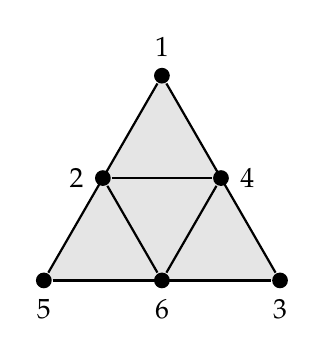
\begin{tikzpicture}[
       thick,
       acteur/.style={
         circle,
         fill=black,
         thick,
         inner sep=2pt,
         minimum size=0.2cm
       }
     ] 

	   \fill[fill=gray!20] (0,0)--(3,0)--(1.5,2.6);

       \node (a1) at (0,0) [acteur,label=below:5]{};
       \node (a2) at (3,0)[acteur,label=below:3]{}; 
       \node (a3) at (1.5,2.6) [acteur,label=above:1]{}; 
       \node (a4) at (0.75,1.3) [acteur,label=left:2]{}; 
       \node (a5) at (2.25,1.3) [acteur,label=right:4]{}; 
       \node (a6) at (1.5,0) [acteur,label=below:6]{};
  
       \draw (a1) -- (a2); 
       \draw (a2) -- (a3); 
       \draw (a1) -- (a3);
       
       \draw (a4) -- (a5);
       \draw (a5) -- (a6);
       \draw (a4) -- (a6);

\end{tikzpicture}
  \caption{The support of a $2$-Cheeger cosystole (The gray triangles represent the four $2$-simplices)}
  \label{figure1:Figure 1}
\end{figure}


Except for the maximal cut-minimal graphs with maximum number of edges we do not know anything about the remaining classes of cut-minimal graphs until now. The following statements now approach this challenge by providing new classes of cut-minimal graphs in general which do not appear as deletions of those largest maximal cut-minimal graphs.

\newpage

\begin{lem}\label{lemma8}
Let \(u_1,\ldots,u_t,s_1,\ldots,s_t\in\mathbb{N}\cup\{0\}\), such that for all \(i=1,\ldots,t\) we have:
\[
u_i+s_i\leq\sum_{\begin{subarray}{l}j=1\\ j\neq i\end{subarray}}^tu_j+s_j,
\]
then we have:
\[
\sum\limits_{i=1}^ts_i(u_i-\sum_{\begin{subarray}{l}j=1\\ j\neq i\end{subarray}}^tu_j)\leq 0
\]
\begin{proof}
If we have
\[
u_i\leq\sum_{\begin{subarray}{l}j=1\\ j\neq i\end{subarray}}^tu_j
\]
for all \(i=1,\ldots,t\), then we are done, since all \(u_i\)'s and \(s_i\)'s are positive. So, let there exist a \(k\in[t]\), such that
\[
u_k>\sum_{\begin{subarray}{l}j=1\\ j\neq k\end{subarray}}^tu_j.
\]
Obviously, there is at most one unique \(u_k\) satisfying this property. Now for all \(i\neq k\) we have:
\[
u_i-\sum_{\begin{subarray}{l}j=1\\ j\neq i\end{subarray}}^tu_j\leq -(u_k-\sum_{\begin{subarray}{l}j=1\\ j\neq k\end{subarray}}^tu_j),
\]
and furthermore we have
\[
s_k<\sum_{\begin{subarray}{l}j=1\\ j\neq k\end{subarray}}^ts_j
\]
by assumption and so we get:
\[
\sum_{\begin{subarray}{l}i=1\\ i\neq k\end{subarray}}^ts_i(u_i-\sum_{\begin{subarray}{l}j=1\\ j\neq i\end{subarray}}^tu_j)\leq-s_k(u_k-\sum_{\begin{subarray}{l}j=1\\ j\neq k\end{subarray}}^tu_j).
\]
Hence, we have:
\[
\sum\limits_{i=1}^ts_i(u_i-\sum_{\begin{subarray}{l}j=1\\ j\neq i\end{subarray}}^tu_j)\leq 0.
\]
\end{proof}
\end{lem}
\begin{prop}
Let \(G=([n],E)\) be a simple graph and let the largest connected component of \(G\) not contain more than \(\frac{n}{2}\) vertices. Then \(G\) is cut-minimal.
\begin{proof}
Let \(C_1,\ldots,C_t\subset [n]\) be the connected components of \(G\) and let \(S\subset [n]\), \(S_i:=S\cap C_i\) and \(U_i:=C_i\setminus S_i\). Then we have:
\[
|E_G(S,[n]\setminus S)|\leq\sum\limits_{i=1}^t|S_i||U_i|
\] 
and
\[
|NE_G(S,[n]\setminus S)|\geq\sum\limits_{i=1}^t(|S_i|\sum_{\begin{subarray}{l}j=1\\ j\neq i\end{subarray}}^t|U_j|).
\]
So, we have to show that
\[
\sum\limits_{i=1}^t|S_i||U_i|\leq\sum\limits_{i=1}^t(|S_i|\sum_{\begin{subarray}{l}j=1\\ j\neq i\end{subarray}}^t|U_j|),
\]
which is equivalent to
\[
\sum\limits_{i=1}^t|S_i|(|U_i|-\sum_{\begin{subarray}{l}j=1\\ j\neq i\end{subarray}}^t|U_j|)\leq 0,
\]
but this follows directly from Lemma \ref{lemma8}, since by the assumption \(|C_i|\leq\frac{n}{2}\) for all \(i\), we have:
\[
|S_i|+|U_i|=|C_i|\leq\sum_{\begin{subarray}{l}j=1\\ j\neq i\end{subarray}}^t|C_j|=\sum_{\begin{subarray}{l}j=1\\ j\neq i\end{subarray}}^t|S_j|+|U_j|.
\]
\end{proof}
\end{prop}

Let us now define and determine the counterpart of the number \(C_{max}(\Delta^{[n]},1)\), namely the minimal number of  edges, a non-cut-minimal graph can have.
\begin{defi}
For any \(n\geq 2\) we define the number:
\[
C_{min}(n):=\min\limits_{\substack{G=([n],E),\\G\text{ is not cut-minimal}}}|E|
\]
\end{defi}
\begin{thm}\label{theorem2}
\(C_{min}(n)=\left\lceil\frac{n}{2}\right\rceil\)
\begin{proof}
We can always find a graph \(G=([n],E)\) with \(\left\lceil\frac{n}{2}\right\rceil\) edges, such that for a vertex \(v\in [n]\) we have
\[
E_G(\{v\},[n]\setminus\{v\})=\left\lceil\frac{n}{2}\right\rceil>\left\lfloor\frac{n-1}{2}\right\rfloor,
\]
so it is not cut-minimal and we have \(C_{min}(n)\leq\left\lceil\frac{n}{2}\right\rceil\).\\
On the other hand if we have a graph \(G=([n],E)\) with \(|E|=\left\lceil\frac{n}{2}\right\rceil-1\), then it must be cut-minimal, since \(\left\lceil\frac{n}{2}\right\rceil-1=\left\lfloor\frac{n-1}{2}\right\rfloor\), so we get \(C_{min}(n)\geq\left\lceil\frac{n}{2}\right\rceil\) and we are done.
\end{proof}
\end{thm}
Obviously, \(\mathcal{C}M(n)\) contains all possible simplices of dimension lower than \(C_{min}(n)\), which leads to the following observation.
\begin{cor}
\(H_k(\mathcal{C}M(n))\cong 0\) for all \(1\leq k\leq\left\lceil\frac{n}{2}\right\rceil-3\)
\begin{proof}
By Theorem \ref{theorem2} \(\mathcal{C}M(n)\) has a full \(k\)-skeleton for all \(k\leq\left\lceil\frac{n}{2}\right\rceil-2\) and we are done. 
\end{proof}
\end{cor}
Since adding a vertex to a cut-minimal graph will never destroy its cut-minimality, we can define the following natural inclusion.
\begin{defi}
For every \(n\in\mathbb{N}\) define:
\begin{align}
i_n\quad :\quad CMG(n)&\longrightarrow CMG(n+1)\notag \\
([n],E)&\longmapsto ([n+1],E)\notag
\end{align}
\end{defi}
Furthermore, we see that maximality of cut-minimal graphs always becomes destroyed by adding a vertex to them.
\begin{prop}
Let \(G\in MAX(n)\), then we have \(i_n(G)\notin MAX(n+1)\).
\begin{proof}
Let \(G=([n],E)\in MAX(n)\). If \(n\) is odd, Theorem \ref{theorem1} gives:
\[
|E|\leq\frac{(n-1)^2}{4}=\frac{n^2-2n+1}{4}<\frac{n^2-n}{4}=\frac{n\frac{n-1}{2}}{2}\quad\text{for }n\geq 3,
\]
so there exists a \(v\in [n]\), such that \(\text{deg}_G(v)<\frac{n-1}{2}\) (*). Now define\\
\(G':=([n+1],E\cup (v,n+1))\) and let \(S\subset [n+1]\), such that \(1\leq |S|\leq\frac{n+1}{2}\), then we have:
\begin{align}
|E_{G'}(S,[n+1]\setminus S)|&\leq |E_G(S\setminus\{n+1\},[n]\setminus S)|+1\notag\\
&\leq\frac{|S|(n-|S|)}{2}+1\notag\\
&=\frac{|S|(n+\frac{2}{|S|}-|S|)}{2}\notag\\
&\leq\frac{|S|(n+1-|S|)}{2},\notag
\end{align}
for all \(S\subset [n+1]\), such that \(|S|\geq 2\). For \(|S|=1\), the upper condition is also satisfied by (*).\\
Hence, \(G'\) is cut-minimal and so we have \(i_n(G)=([n+1],E)\notin MAX(n+1)\).\\
If \(n\) is even, define \(G':=([n+1],E\cup (v,n+1))\) for some arbitrary \(v\in [n]\). Then by the same calculations as in the first part, we have
\[
|E_{G'}(S,[n+1]\setminus S)|\leq\frac{|S|(n+1-|S|)}{2},
\]
for all \(S\subset [n+1]\), such that \(|S|\geq 2\), and for \(|S|=1\) we have:
\begin{align}
|E_{G'}(S,[n+1]\setminus S)|&\leq\text{max}\{\text{deg}_{G'}(v)\text{ : }v\in[n+1]\}\notag\\
&=\left\lfloor\frac{n-1}{2}\right\rfloor +1\notag\\
&=\frac{n-2}{2}+1=\frac{n}{2}=\frac{(n+1)-1}{2}.\notag
\end{align}
Hence, \(G'\) is cut-minimal and \(i_n(G)\notin MAX(n+1)\).
\end{proof}
\end{prop}

\section{Cheeger graphs}
In this chapter we want to recall the notion of Cheeger graphs and the first Cheeger constant of a simplex as introduced in \cite{1} but then not try to determine the Cheeger constant for certain simplices more precisely but investigate the combinatorial structure of Cheeger graphs and develop some methods which might help to check if a given cut-minimal graph is a Cheeger graph or not.

\subsection{Basic definitions and properties}
The following definition is completely adopted from \cite{1}.
\begin{defi}\label{definition1}
Consider a graph \(G=([n],E)\), then we set:
\begin{small}
\[
T(G):=\{(v,e)\: :\: v\in [n]\text{, }e=(w,u)\in E\text{, }v\notin e\text{, }|\{(v,w),(v,u),(w,u)\}\cap E\}|\text{ is odd}\}.
\]
\end{small}
We have:
\[
|T(G)|=\sum\limits_{e\in E}t(e),
\]
where for an edge \(e=(v,w)\), we set
\[
t(e):=\sum\limits_{u\in[n]\text{ : }u\neq v,w}\tau_e(u),
\]
with
\begin{equation}
\tau_e(u):=
\begin{cases}
1,&\text{ if }(v,u),(w,u)\notin E\notag\\
\frac{1}{3},&\text{ if }(v,u),(w,u)\in E\notag\\
0,&\text{ otherwise}\notag
\end{cases}
\end{equation}
Furthermore, we adopt the number:
\[
h(G):=\frac{|T(G)|}{|E|}
\]
and call a cut-minimal graph \(G=([n],E)\) a \textbf{Cheeger graph}, if
\[
h(G)=\min\limits_{G'\in CMG(n)}h(G').
\]
The \textbf{first Cheeger constant of a simplex} \(h_1(\Delta^{[n]})\) is then defined by:
\[
h_1(\Delta^{[n]}):=h(G)
\]
where \(G\) is some Cheeger graph on \(n\) vertices.
\end{defi}
We already know by \cite{1} that \(\frac{n}{3}\leq h_1(\Delta{[n]})\leq\left\lceil\frac{n}{3}\right\rceil\) and the lower bound is archieved if \(n\) is not a power of \(2\). If two graphs \(G\) and \(G'\) belong to the same isomorphism class, we obviously have \(|T(G)|=|T(G')|\) and \(h(G)=h(G')\), so taking up the example from the preceding section, Figure 2 shows the numbers \(h(G)\) for all cut-minimal graphs on \(6\) vertices with the same partially ordering as in Figure 1 and we can see that there is one Cheeger graph attaining the Cheeger constant \(\frac{8}{4}\).

\begin{figure}[ht]
\centering
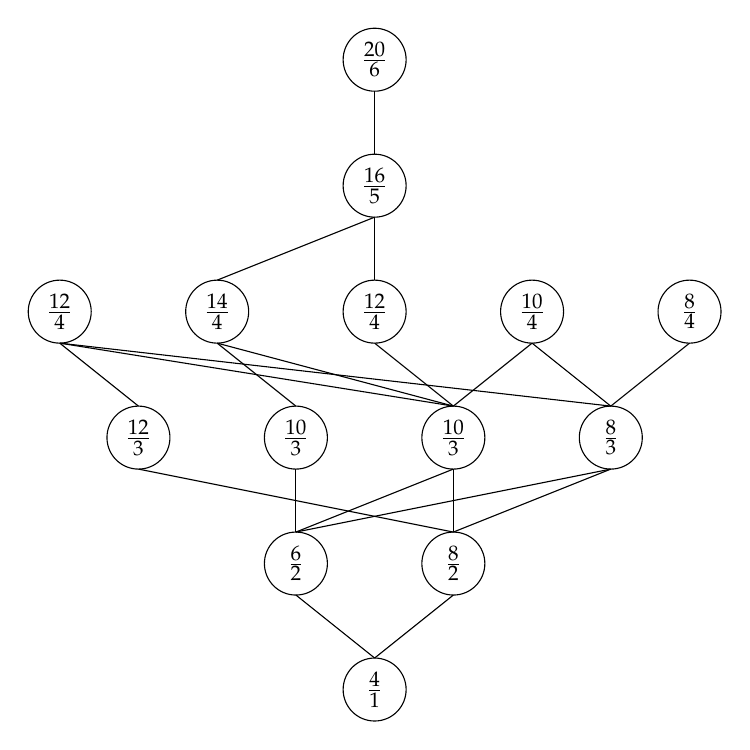
\begin{tikzpicture}
  [scale=.04,auto=left]
  
  \def\X{40}
  \def\Y{0}
  
  \def\x{\X -10}
  \def\y{\Y}
  
  \draw  (\x +10,\y +5) circle [radius=10cm] node {$\frac{4}{1}$};

  \def\x{\X -35}
  \def\y{\Y +40}
    
  \draw  (\x +10,\y +5) circle [radius=10cm] node {$\frac{6}{2}$};
  
  \draw  (\x +10,\y -5) -- (\x +35,\y -25);
  
  \def\x{\X +15}
  \def\y{\Y +40}
    
  \draw  (\x +10,\y +5) circle [radius=10cm] node {$\frac{8}{2}$};
  
  \draw  (\x +10,\y -5) -- (\x -15,\y -25);
  
  \def\x{\X -85}
  \def\y{\Y +80}
    
  \draw  (\x +10,\y +5) circle [radius=10cm] node {$\frac{12}{3}$};
  
  \draw  (\x +10,\y -5) -- (\x +110,\y -25);
  
  \def\x{\X -35}
  \def\y{\Y +80}
    
  \draw  (\x +10,\y +5) circle [radius=10cm] node {$\frac{10}{3}$};
  
  \draw  (\x +10,\y -5) -- (\x +10,\y -25);
  
  \def\x{\X +15}
  \def\y{\Y +80}
    
  \draw  (\x +10,\y +5) circle [radius=10cm] node {$\frac{10}{3}$};
  
  \draw  (\x +10,\y -5) -- (\x +10,\y -25);
  \draw  (\x +10,\y -5) -- (\x -40,\y -25);
  
  \def\x{\X +65}
  \def\y{\Y +80}
    
  \draw  (\x +10,\y +5) circle [radius=10cm] node {$\frac{8}{3}$};
  
  \draw  (\x +10,\y -5) -- (\x -40,\y -25);
  \draw  (\x +10,\y -5) -- (\x -90,\y -25);
  
  \def\x{\X -110}
  \def\y{\Y +120}
    
  \draw  (\x +10,\y +5) circle [radius=10cm] node {$\frac{12}{4}$};
  
  \draw  (\x +10,\y -5) -- (\x +35,\y -25);
  \draw  (\x +10,\y -5) -- (\x +135,\y -25);
  \draw  (\x +10,\y -5) -- (\x +185,\y -25);
  
  \def\x{\X -60}
  \def\y{\Y +120}
    
  \draw  (\x +10,\y +5) circle [radius=10cm] node {$\frac{14}{4}$};
  
  \draw  (\x +10,\y -5) -- (\x +35,\y -25);
  \draw  (\x +10,\y -5) -- (\x +85,\y -25);
  
  \def\x{\X -10}
  \def\y{\Y +120}
    
  \draw  (\x +10,\y +5) circle [radius=10cm] node {$\frac{12}{4}$};
  
  \draw  (\x +10,\y -5) -- (\x +35,\y -25);
  
  \def\x{\X +40}
  \def\y{\Y +120}
    
  \draw  (\x +10,\y +5) circle [radius=10cm] node {$\frac{10}{4}$};
  
  \draw  (\x +10,\y -5) -- (\x +35,\y -25);
  \draw  (\x +10,\y -5) -- (\x -15,\y -25);
  
  \def\x{\X +90}
  \def\y{\Y +120}
    
  \draw  (\x +10,\y +5) circle [radius=10cm] node {$\frac{8}{4}$};
  
  \draw  (\x +10,\y -5) -- (\x -15,\y -25);
  
  \def\x{\X -10}
  \def\y{\Y +160}
    
  \draw  (\x +10,\y +5) circle [radius=10cm] node {$\frac{16}{5}$};
  
  \draw  (\x +10,\y -5) -- (\x +10,\y -25);
  \draw  (\x +10,\y -5) -- (\x -40,\y -25);
  
  \def\x{\X -10}
  \def\y{\Y +200}
    
  \draw  (\x +10,\y +5) circle [radius=10cm] node {$\frac{20}{6}$};
  
  \draw  (\x +10,\y -5) -- (\x +10,\y -25);
\end{tikzpicture}
  \caption{The numbers \(h(G)\) for all cut-minimal graphs on 6 vertices}
  \label{figure2:Figure 2}
\end{figure}


\subsection{Deletions and additions of edges}
We will now investigate how the set \(T(G)\) (and so the constant \(h(G)\) as well) changes when we delete or add one or more edges in a given graph \(G\). This will give us some methods to determine that a given graph satisfying certain conditions is not a Cheeger graph.
\begin{defi}
Let \(G=([n],E)\) be a simple graph. For an edge \(e\in E\) we define the numbers:
\[
\psi_e^G:=|\{e'\in E\: :\: e'\text{ and }e\text{ share a vertex}\}|,
\]
where two edges \(e=(v_1,v_2)\) and \(e'=(v_3,v_4)\) are said to be sharing a vertex, if \(|(v_1,v_2)\cap (v_3,v_4)|=1\) and
\[
\phi_e^G:=|\{A\subseteq E\: :\: A\text{ is a triangle in }G\text{ and }e\in A\}|,
\]
where a triangle is a set of the type \(A=\{(v_1,v_2),(v_2,v_3),(v_3,v_1)\}\). If \(G\) contains no triangle, which is equivalent to \(\sum\limits_{e\in E}\phi_e^G=0\), then we call \(G\) \textbf{triangle-free}.
\end{defi}
\begin{lem}\label{lemma2}
Let \(G=([n],E)\) be a cut-minimal graph and \(e\in E\), then we have:
\begin{equation}
\psi_e^G\leq
\begin{cases}
n-3,&\text{ for }n\text{ odd}\notag\\
n-4,&\text{ for }n\text{ even}\notag
\end{cases}
\end{equation}
and
\begin{equation}
\phi_e^G\leq
\begin{cases}
\frac{n-3}{2},&\text{ for }n\text{ odd}\notag\\
\frac{n-4}{2},&\text{ for }n\text{ even}\notag
\end{cases}
\end{equation}
\begin{proof}
Let \(e:=(v_1,v_2)\), then we have \(\text{deg}_G(v_1),\text{deg}(v_2)\leq\left\lfloor\frac{n-1}{2}\right\rfloor\), so we get:
\[
\psi_e^G=\text{deg}_G(v_1)+\text{deg}_G(v_2)-2\leq2\left\lfloor\frac{n-1}{2}\right\rfloor-2
\]
Since \(2\left\lfloor\frac{n-1}{2}\right\rfloor=n-1\) for \(n\) odd and \(n-2\) for \(n\) even we get the claimed result.\\
The second part follows directly from the first one, since for each triangle containing \(e\), we have exactly two edges sharing a vertex with \(e\).
\end{proof}
\end{lem}
Since a Cheeger graph \(G\) can be characterized by the property that neither deleting edges from it nor adding edges to it (provided that the corresponding graph is still cut-minimal) nor a combination of both actions can decrease the number \(h(G)\), it might be helpful to know more about how those actions change \(h(G)\). The next Lemma gives exactly this information and the following statements then develop conditions which being satisfied by a certain graph guarantee that it is not a Cheeger graph.
\begin{lem}\label{lemma1}
Let \(G=([n],E)\) be a simple graph, \(e\in E\) and \(e'\in NE_G([n],[n])\). Then we have:
\begin{enumerate}
\item \(|T(G)|\leq |E|(n-2)-2\psi_e^G+2\phi_e^G\)
\item \(|T(G_e)|=|T(G)|-(n-2)+2(\psi_e^G-2\phi_e^G)\)
\item \(|T(G^{e'})|=|T(G)|+(n-2)-2(\psi_{e'}^{G^{e'}}-2\phi_{e'}^{G^{e'}})\)
\end{enumerate}
\begin{proof}
(1) The maximum number \(|T(G)|\) can become is obviously \(|E|(n-2)\), namely in the case when no two edges share a vertex. Now for an edge\\
\(e=(v_1,v_2)\in E\) contained in a triangle \(\{(v_1,v_2),(v_1,v_3),(v_2,v_3)\}\), we have \(\tau_e(v_3)=\frac{1}{3}\) instead of \(1\), so \(t(e)\) decreases at least by \(\frac{2}{3}\).
By 3 edges participating at each triangle, we then overall lose at least \(2\phi_e^G\).\\
If we have two edges \((v_1,v_2),(v_2,v_3)\in E\), such that \((v_1,v_3)\notin E\), meaning two edges which share a vertex but which are not contained in the same triangle, then we get \(\tau_{(v_1,v_2)}(v_3)=\tau_{(v_2,v_3)}(v_1)=0\) instead of \(1\), so overall we lose at least \(2(\psi_e^G-2\phi_e^G)\), since \(\psi_e^G-2\phi_e^G\) is the number of edges which share a vertex with \(e\) but which are not contained in the same triangle with \(e\).\\
All in all we get:
\[
|T(G)|\leq|E|(n-2)-2\phi_e^G-2(\psi_e^G-2\phi_e^G)=|E|(n-2)-2\psi_e^G+2\phi_e^G
\]
(2) The maximum number by which \(|T(G)|\) can decrease when deleting \(e\) from \(G\) is \(n-2\). This is the case when \(e\) is not connected to the rest of the graph. We do not have to consider the case when \(e\) is contained in a triangle because even though \(t(e)\) is smaller than \(n-2-\frac{2}{3}\) then, the numbers \(t(e')\) and \(t(e'')\) refering to the other two edges \(e'\) and \(e''\) contained in the triangle also decrease by \(\frac{1}{3}\) when deleting \(e\).
So, we still have to consider the case, when we have an edge \(e'\) sharing a vertex with \(e\) but not being contained in the same triangle with \(e\). Then \(|T(G)|\) decreases by one less than \(n-2\) and even increases by 1 when deleting \(e\), since \(t(e')\) increases by 1.\\
Hence, we get:
\[
|T(G_e)|=|T(G)|-(n-2)+2(\psi_e^G-2\phi_e^G)
\]
(3) By part (2) of this Lemma we have:
\[
|T(G)|=|T(G_{e'}^{e'})|=|T(G^{e'})|-(n-2)+2(\psi_{e'}^{G^{e'}}-2\phi_{e'}^{G^{e'}})
\]
which is equivalent to:
\[
|T(G^{e'})|=|T(G)|+(n-2)-2(\psi_{e'}^{G^{e'}}-2\phi_{e'}^{G^{e'}}).
\]
\end{proof}
\end{lem}
\begin{prop}\label{proposition1}
Let \(G=([n],E)\) be a simple graph. If there exists an edge \(e\in E\), such that \(2(|E|-1)\psi_e^G-2(2|E|-1)\phi_e^G<0\), then we have \(h(G_e)<h(G)\).
\begin{proof}
By Lemma \ref{lemma1} (1) we get:
\begin{doublespace}
\begin{align}
&\quad\quad\quad\:\, |E|(n-2)-(2\psi_e^G-2\phi_e^G)\geq |T(G)|\notag\\
&\Longleftrightarrow\quad |E||T(G)|-|E|(n-2)+(2\psi_e^G-2\phi_e^G)\leq |T(G)|(|E|-1)\notag\\
&\Longleftrightarrow\quad \frac{|E||T(G)|-|E|(n-2)+(2\psi_e^G-2\phi_e^G)}{|E|(|E|-1)}\leq\frac{|T(G)|(|E|-1)}{|E|(|E|-1)}\notag\\
&\Longleftrightarrow\quad \frac{|T(G)|-(n-2)}{|E|-1}+\frac{2\psi_e^G-2\phi_e^G}{|E|(|E|-1)}\leq\frac{|T(G)|}{|E|}=h(G)
\end{align}
\end{doublespace}
and by Lemma \ref{lemma1} (2) we get:
\begin{align}
h(G_e)=\frac{|T(G)|-(n-2)}{|E|-1}+\frac{2\psi_e^G-4\phi_e^G}{|E|-1}
\end{align}
Now consider:
\begin{doublespace}
\begin{align}
&\quad\quad\quad\:\, 2(|E|-1)\psi_e^G-2(2|E|-1)\phi_e^G<0\notag\\
&\Longleftrightarrow\quad 2(|E|-1)\psi_e^G-(4|E|-2)\phi_e^G<0\notag\\
&\Longleftrightarrow\quad 2(|E|-1)\psi_e^G-4|E|\phi_e^G+2\phi_e^G<0\notag\\
&\Longleftrightarrow\quad 2|E|\psi_e^G-4|E|\phi_e^G<2\psi_e^G-2\phi_e^G\notag\\
&\Longleftrightarrow\quad \frac{2\psi_e^G-4\phi_e^G}{|E|-1}<\frac{2\psi_e^G-2\phi_e^G}{|E|(|E|-1)}\notag
\end{align}
\end{doublespace}
So, by (1) and (2) we have:
\[
h(G_e)<h(G)
\]
\end{proof}
\end{prop}
\begin{expl}
Let \(G=([n],E)\) be a simple graph containing a triangle, which is only connected to the rest of the graph via one vertex or isolated, meaning a set \(\{(v_1,v_2),(v_2,v_3),(v_1,v_3)\}\subseteq E\), such that \(\text{deg}_G(v_1)=\text{deg}_G(v_2)=2\), then \(G\) is not a Cheeger graph as follows. We set \(e:=(v_1,v_2)\), then we have \(\phi_e^G=1\) and \(\psi_e^G=2\). This gives us:
\[
2(|E|-1)\psi_e^G-2(2|E|-1)\phi_e^G=4(|E|-1)-2(2|E|-1)=-2<0
\]
and by Proposition \ref{proposition1} we get:
\[
h(G_e)<h(G),
\]
so \(G\) can not be a Cheeger graph.
\end{expl}
Now we want to generalize the second and third part of Lemma \ref{lemma1} to a situation where we consider more than only one edge being deleted or added.
\begin{lem}\label{lemma3}
Let \(G=([n],E)\) be a simple graph and \(e_1,\ldots,e_k\in E\), then we have:
\[
|T(G_{e_1,\ldots,e_k})|=|T(G)|-k(n-2)+2(\sum\limits_{i=1}^k\psi_{e_i}^{G_{e_1,\ldots,e_{i-1}}}-2\sum\limits_{i=1}^k\phi_{e_i}^{G_{e_1,\ldots,e_{i-1}}})
\]
In this formula we set \(G_{e_0}=G\) to avoid writing it in a more complicated way.\\
For \(e_1,\ldots,e_k\in NE_G([n],[n])\) we have:
\[
|T(G^{e_1,\ldots,e_k})|=|T(G)|+k(n-2)-2(\sum\limits_{i=1}^k\psi_{e_i}^{G^{e_1,\ldots,e_i}}-2\sum\limits_{i=1}^k\phi_{e_i}^{G^{e_1,\ldots,e_i}})
\]
\begin{proof}
By Lemma \ref{lemma1} (2) we get:
\begin{align}
|T(G_{e_1,\ldots,e_k})|&=|T(G_{e_1,\ldots,e_{k-1}})|-(n-2)+2(\psi_{e_k}^{G_{e_1,\ldots,e_{k-1}}}-2\phi_{e_k}^{G_{e_1,\ldots,e_{k-1}}})\notag\\
&=|T(G_{e_1,\ldots,e_{k-2}})|-(n-2)+2(\psi_{e_{k-1}}^{G_{e_1,\ldots,e_{k-2}}}-2\phi_{e_{k-1}}^{G_{e_1,\ldots,e_{k-2}}})\notag\\
&\quad-(n-2)+2(\psi_{e_k}^{G_{e_1,\ldots,e_{k-1}}}-2\phi_{e_k}^{G_{e_1,\ldots,e_{k-1}}})\notag\\
&=|T(G_{e_1,\ldots,e_{k-2}})|-2(n-2)\notag\\
&\quad+2(\psi_{e_{k-1}}^{G_{e_1,\ldots,e_{k-2}}}+\psi_{e_k}^{G_{e_1,\ldots,e_{k-1}}}-2(\phi_{e_{k-1}}^{G_{e_1,\ldots,e_{k-2}}}+\phi_{e_k}^{G_{e_1,\ldots,e_{k-1}}}))\notag
\end{align}
so inductively we have:
\[
|T(G_{e_1,\ldots,e_k})|=|T(G)|-k(n-2)+2(\sum\limits_{i=1}^k\psi_{e_i}^{G_{e_1,\ldots,e_{i-1}}}-2\sum\limits_{i=1}^k\phi_{e_i}^{G_{e_1,\ldots,e_{i-1}}})
\]
The second part works analogously using Lemma \ref{lemma1} (3). 
\end{proof}
\end{lem}
\begin{prop}\label{proposition2}
Let \(G=([n],E)\) be a simple graph. If there exist edges \(e_1,\ldots,e_k\in E\) and \(e\in E\) such that:
\[
\frac{2(\sum\limits_{i=1}^k\psi_{e_i}^{G_{e_1,\ldots,e_{i-1}}}-2\sum\limits_{i=1}^k\phi_{e_i}^{G_{e_1,\ldots,e_{i-1}}})}{|E|-k}<\frac{k(2\psi_e^G-2\phi_e^G)}{|E|(|E|-k)},
\]
then we have:
\[
h(G_{e_1,\ldots,e_k})<h(G)
\]
\begin{proof}
By Lemma \ref{lemma1} (1) we get:
\begin{doublespace}
\begin{align}
&\quad\quad\quad\:\, |E|(n-2)-(2\psi_e^G-2\phi_e^G)\geq |T(G)|\notag\\
&\Longleftrightarrow\quad |E||T(G)|-k|E|(n-2)+k(2\psi_e^G-2\phi_e^G)\leq |T(G)|(|E|-k)\notag\\
&\Longleftrightarrow\quad \frac{|E||T(G)|-k|E|(n-2)+k(2\psi_e^G-2\phi_e^G)}{|E|(|E|-k)}\leq\frac{|T(G)|(|E|-k)}{|E|(|E|-k)}\notag\\
&\Longleftrightarrow\quad \frac{|T(G)|-k(n-2)}{|E|-k}+\frac{k(2\psi_e^G-2\phi_e^G)}{|E|(|E|-k)}\leq\frac{|T(G)|}{|E|}=h(G)
\end{align}
\end{doublespace}
and Lemma \ref{lemma3} gives us:
\[
h(G_{e_1,\ldots,e_k})=\frac{|T(G)|-k(n-2)}{|E|-k}+\frac{2(\sum\limits_{i=1}^k\psi_{e_i}^{G_{e_1,\ldots,e_{i-1}}}-2\sum\limits_{i=1}^k\phi_{e_i}^{G_{e_1,\ldots,e_{i-1}}})}{|E|-k}
\]
So, by (3) and the assumption we have:
\[
h(G_{e_1,\ldots,e_k})<h(G)
\]
\end{proof}
\end{prop}

\subsection{Adding vertices to Cheeger graphs}
After we studied how adding or deleting edges in a cut-minimal graph \(G\) affects its constant \(h(G)\) we are now interested in the consequences of adding a vertex to \(G\). We will find out that in the most cases the property of being a Cheeger graph will be destroyed by this action. Using this knowledge we can construct a lower bound on the number of edges in Cheeger graphs holding in the most cases.
\begin{lem}\label{lemma4}
Let \(G=([n],E)\) be a cut-minimal graph, then we have:
\[
h(i_n(G))=h(G)+1
\]
\begin{proof}
Adding an isolated vertex to a graph \(G=([n],E)\) obviously increases \(|T(G)|\) by \(|E|\), so we get:
\[
h(i_n(G))=\frac{|T(G)|+|E|}{|E|}=\frac{|T(G)|}{|E|}+\frac{|E|}{|E|}=h(G)+1
\]
\end{proof}
\end{lem}
A direct consequence of this relation is that if \(n\) is not divisible by 3, Cheeger graphs in \(CMG(n)\) can not appear as an embedding of graphs from \(CMG(n-1)\).
\begin{prop}\label{proposition4}
For all \(G\in CMG(n)\), such that \(3\nmid n\) the graph\\
\(i_n(G)\in CMG(n+1)\) is not a Cheeger graph.
\begin{proof}
We only need to consider Cheeger graphs in \(CMG(n)\), since for any\\
\(G\in CMG(n)\) which is not a Cheeger graph, there exists a graph \(G'\in CMG(n)\), such that \(h(G')<h(G)\), so by Lemma \ref{lemma4} we get:
\[
h(i_n(G'))=h(G')+1<h(G)+1=h(i_n(G))
\]
Let now \(G\in CMG(n)\) be a Cheeger graph. Then by a result from \cite{1} we get:
\[
\frac{n}{3}\leq h(G)\leq\left\lceil\frac{n}{3}\right\rceil
\]
which implies that:
\[
h(i_n(G))=h(G)+1\geq\frac{n}{3}+1\geq\left\lceil\frac{n+1}{3}\right\rceil,
\]
where the last inequality is sharp if and only if \(3\nmid n\).\\
So, if \(3\nmid n\) then \(i_n(G)\) is not a Cheeger graph, since by \cite{1} we have:
\[
h_1(\Delta^{[n+1]})\leq\left\lceil\frac{n+1}{3}\right\rceil<h(i_n(G))
\]
\end{proof}
\end{prop}
We even have a similar version of the previous statement if \(n\) is divisible by 3 with the restriction that \(n+1\) must not be a power of 2.
\begin{prop}\label{proposition5}
Let \(G\in CMG(n)\), such that \(3\mid n\) and \(n+1\neq2^t\) for some \(t\in\mathbb{N}\). Then \(i_n(G)\) is not a Cheeger graph.
\begin{proof}
Since \(n\) is divisible by 3 we have \(h(G)=\frac{n}{3}\) by \cite{1} and so we get\\
\(h(i_n(G))=\frac{n}{3}+1\) by Lemma \ref{lemma4}. Now, since \(n+1\) is not a power of 2 we also know that \(h_1(\Delta^{[n+1]})=\frac{n+1}{3}\) by \cite{1}. Hence, we have:
\[
h(i_n(G))>h_1(\Delta^{[n+1]})
\]
\end{proof}
\end{prop}
Combining the last two statements, we can calculate a lower bound for the number of edges in Cheeger graphs, except for the case when the number of vertices \(n\) is a power of 2 and \(n-1\) is divisible by 3.
\begin{prop}
Let \(G=([n],E)\) be a Cheeger graph, such that \(n\) is not a power of 2 or \(n-1\) is not divisible by 3. Then we have \(|E|\geq\left\lceil\frac{n-1}{2}\right\rceil\).
\begin{proof}
Assume we have \(|E|<\left\lceil\frac{n-1}{2}\right\rceil\). Then by Theorem \ref{theorem2} and since \(G\) must contain an isolated vertex, there exists a graph \(G'\in CMG(n-1)\), such that \(i_{n-1}(G')=G\). Now if we have \(n\neq 2^t\) for some \(t\in\mathbb{N}\), then \(G\) is not a Cheeger graph, since we either get \(3\nmid n-1\) and we are done by Proposition \ref{proposition4} or we get \(3\mid n-1\) and we are done by Proposition \ref{proposition5}. On the other hand, if we have \(n=2^t\) but \(3\nmid n-1\), then we immediately see that \(G\) is not a Cheeger graph by Proposition \ref{proposition4}.
\end{proof}
\end{prop}
% Chapter 6

\chapter{Alternative generalizations of the classical Cheeger constant}

\label{Chapter6}

In the introduction we defined the generalization of the classical Cheeger constant which was already introduced by Linial and Meshulam (see \cite{2}) and later independently by Gromov (see \cite{3}). But that notion is not the only way to generalize the classical Cheeger constant and we do not even know if it is the "best" way to generalize it, concerning the information these constants give about the stability of connectedness of simplicial complexes. In Chapter \ref{Chapter2} we saw that there is a close connection between the cosystolic norm of a cochain and the hitting number of a certain family of cycles, so we will use this connection to introduce other notions of the Cheeger constant which attain the same value as our earlier notion on a large family of complexes, but might be easier to determine in certain situations. These other notions were introduced by Kozlov (see \cite{13}).

\section{Disjoint cycle expansion and hitting expansion}

\begin{defi}\label{definition411}
Let \(X\) be a simplicial complex and \(k\geq 1\). Furthermore, let \(\mathcal{F}\subset C_k(X)\) be a family of cycles, such that their supports are pairwise disjoint (i.e. \(\supp(F)\cap\supp(F')=\emptyset\) for all \(F,F'\in\mathcal{F}\), satisfying \(F\neq F'\)) and let
\begin{small}
\[
P(\mathcal{F})\coloneqq\{\varphi\in C^k(X):|\supp(\varphi)\cap\supp(F)|=1\text{ for all }F\in\mathcal{F}\text{ and }\supp(\varphi)\subset\bigcup\limits_{F\in\mathcal{F}}\supp(F)\}
\]
\end{small}
denote the set of all cochains constructed by all possible choices of one simplex per cycle in the family \(\mathcal{F}\). Then we define
\[
\gamma_{\mathcal{F}}\coloneqq\frac{\min\limits_{\varphi\in P(\mathcal{F})}\|\delta^k(\varphi)\|}{|\mathcal{F}|}
\]
and we call
\[
\gamma_k(X)\coloneqq\min\limits_{\mathcal{F}\in\mathfrak{C}}\gamma_{\mathcal{F}}
\]
the \(k\)-th \textbf{disjoint cycle expansion}\index{Disjoint cycle expansion} of \(X\), where
\begin{small}
\[
\mathfrak{C}\coloneqq\{\mathcal{F}\subset C_k(X):F\text{ is a cycle and }\supp(F)\cap\supp(F')=\emptyset\text{ for all }F,F'\in\mathcal{F}\:(F\neq F')\}
\]
\end{small}
is the collection of all families of cycles in \(C_k(X)\) with pairwise disjoint supports.
\end{defi}

\begin{defi}\label{definition412}
Let \(X\) be a simplicial complex and \(k\geq 1\). Furthermore, let \(\mathcal{F}\subset C_k(X)\) be an arbitrary family of cycles and let
\[
P'(\mathcal{F})\coloneqq\{\varphi\in C^k(X):|\supp(\varphi)\cap\supp(F)|\text{ is odd for all }F\in\mathcal{F}\}
\]
Then we define
\[
\rho_{\mathcal{F}}\coloneqq\frac{\min\limits_{\varphi\in P'(\mathcal{F})}\|\delta^k(\varphi)\|}{\tau(\mathcal{F})}
\]
and we call
\[
\rho_k(X)\coloneqq\min\limits_{\mathcal{F}\in\mathfrak{C}}\rho_{\mathcal{F}}
\]
the \(k\)-th \textbf{hitting expansion}\index{Hitting expansion} of \(X\), where
\[
\mathfrak{C}\coloneqq\{\mathcal{F}\subset C_k(X):F\text{ is a cycle, for all }F\in\mathcal{F}\}
\]
is the collection of all families of cycles in \(C_k(X)\).
\end{defi}

\section{Relations to the Cheeger constant}

\begin{prop}\label{proposition411}
Let \(X\) be a simplicial complex and \(k\geq 1\), then we have:
\[
h_k(X)\leq\rho_k(X)\leq\gamma_k(X)
\]
\begin{proof}
Let \(\mathcal{F}\subset C_k(X)\) be a family of cycles with pairwise disjoint supports and \(\varphi\in P(\mathcal{F})\). Then we have \(\varphi\in P'(\mathcal{F})\) and \(\tau(\mathcal{F})=|\mathcal{F}|\) and we immediately get \(\rho_{\mathcal{F}}\leq\gamma_{\mathcal{F}}\), so we have \(\rho_k(X)\leq\gamma_k(X)\). Let now \(\mathcal{F}\subset C_k(X)\) be an arbitrary family of cycles and \(\varphi\in P'(\mathcal{F})\). Then we have \(\langle\varphi,F\rangle=1\) for all \(F\in\mathcal{F}\) so we can use the cycle detection theorem and we get \(\|\varphi\|_{csy}\geq\tau(\mathcal{F})\). This implies \(\|\varphi\|_{exp}\leq\rho_{\mathcal{F}}\) and we have \(h_k(X)\leq\rho_k(X)\).
\end{proof}
\end{prop}

We will now show that the first disjoint cycle expansion (and thus also the first hitting expansion) of the simplex on \(n\) vertices equals the first Cheeger constant whenever \(n\) is not a power of \(2\).

\begin{thm}\label{theorem421}
Let \(n\) not be a power of \(2\), then we have:
\[
\gamma_1(\Delta^{[n]})=\rho_1(\Delta^{[n]})=\frac{n}{3}
\] 
\begin{proof}
Since \(n\) is not a power of \(2\) we can write it as \(n=c(2t+1)\). Now consider the staircase graph \(G_n(\lambda)\) given by the partition \(\lambda=c\cdot\text{cor}(t)\). For the definition of staircase graphs and partitions, see \cite{1}. Since \(G_n(\lambda)\) is bipartite we can partition the vertices of \(G_n(\lambda)\) as \([n]=A\cup B\cup C\), with \(A=\{v_1,\ldots,v_{ct}\}\), \(B=\{w_1,\ldots,w_{ct}\}\) and \(C=\{x_1,\ldots,x_c\}\), such that \(C\) is the set of all isolated vertices, and all edges of \(G_n(\lambda)\) are contained in \(E_{G_n(\lambda)}(A,B)\). Construct a family of cycles in \(C_1(\Delta^{[n]})\) with pairwise disjoint supports as follows:\\
For all edges \((v_i,w_j)\) satisfying \(i+j\leq ct\), such that \((v_{ct-j+1},w_{ct-i+1})\) is not an edge in \(G_n(\lambda)\) consider the cycle
\[
C_{ij}\coloneqq (v_i,w_j)+(v_{ct-j+1},w_{ct-i+1})+(v_i,v_{ct-j+1})+(w_j,w_{ct-i+1})
\]
For all edges \(e_{ij}=(v_i,w_j)\) satisfying \(i+j\leq ct+1\), such that \(e'_{ij}=(v_{ct-j+1},w_{ct-i+1})\) is also an edge in \(G_n(\lambda)\) (for \(i+j=ct+1\) they are equal), the set
\[
D\coloneqq\{e_{ij}, e'_{ij}:i+j\leq ct+1\text{, }e_{ij}\text{ and }e'_{ij}\text{ are edges in }G_n(\lambda)\}
\] can be partitioned into \(t\) sets \(B_1,\ldots,B_t\), each containing \(c^2\) edges:
\[
B_k\coloneqq\{(v_i,w_j):(k-1)c+1\leq i\leq kc\text{, }c(t-k)+1\leq j\leq c(t-k+1)\}
\]
Now, each vertex from \(A\cup B\) is only contained in edges from exactly one of the sets \(B_k\). This means that for any \(l=1,\ldots,c\) and any pair of edges \((v_i,w_j)\in B_{k_1}\) and \((v_{i'},w_{j'})\in B_{k_2}\) (\(k_1\neq k_2\)) the supports of the cycles \((v_i,w_j)+(v_i,x_l)+(w_j,x_l)\) and \((v_{i'},w_{j'})+(v_{i'},x_l)+(w_{j'},x_l)\) are disjoint. Furthermore, each set \(B_k\) itself is a complete balanced bipartite graph (i.e. a graph in which each of the \(c\) vertices from \(A\) is adjacent to each of the \(c\) vertices from \(B\)) so we can partition it into \(c\) sets \(B_k^1,\ldots,B_k^c\), such that all edges in \(B_k^l\) are disjoint, for every \(l=1,\ldots,c\). Thus, the supports of the cycles \((v_i,w_j)+(v_i,x_l)+(w_j,x_l)\) are pairwise disjoint for all \((v_i,w_j)\in B_k^l\). The family of all these cycles united with the cycles \(C_{ij}\) we defined before gives a family of cycles with pairwise disjoint supports, such that every edge of \(G_n(\lambda)\) is contained in exactly one cycle and every cycle containes exactly one of the edges from \(G_n(\lambda)\). Since the number of cycles in this family equals the number of edges in \(G_n(\lambda)\) and we know that we have \(h(G_n(\lambda))=\frac{n}{3}\) by \cite{1} (Theorem 4.2.) we get \(\gamma_1(\Delta^{[n]})\leq\frac{n}{3}\) and by Proposition \ref{proposition411} we have \(\gamma_1(\Delta^{[n]})=\rho_1(\Delta^{[n]})=\frac{n}{3}\).
\end{proof}
\end{thm}

\begin{expl}

Let \(n=10\) and consider the staircase graph \(G_{10}(\lambda)\) with \(\lambda=2\cdot\text{cor}(2)\) as shown in Figure \ref{figure13:Figure 13} (\(v_i\) and \(w_j\) are adjacent if and only if there is a box in column \(i\) and row \(j\) and the \(x_i\)'s are isolated vertices). Then, intuitively speaking, for every edge represented by a box for which there is no box on the other side of the diagonal
\[
(v_1,w_4),(v_2,w_3),(v_3,w_2),(v_4,w_1)
\]
we can "use" the missing boxes to construct cycles for these edges as we did in the first part of the proof of Theorem \ref{theorem421}. This means, we get the family of cycles:
\begin{align}
\{&(v_1,w_1)+(v_4,w_4)+(v_1,v_4)+(w_1,w_4),(v_2,w_2)+(v_3,w_3)+(v_2,v_3)+(w_2,w_3),\notag\\
&(v_1,w_2)+(v_3,w_4)+(v_1,v_3)+(w_2,w_4),(v_2,w_1)+(v_4,w_3)+(v_2,v_4)+(w_1,w_3)\}\notag
\end{align}
For the remaining edges, according to the second part of the proof we use the isolated vertices to construct cycles and we get the family of cycles:
\begin{align}
\{&(v_1,w_4)+(v_1,x_1)+(w_4,x_1),(v_2,w_3)+(v_2,x_1)+(w_3,x_1),\notag\\
&(v_3,w_2)+(v_3,x_1)+(w_2,x_1),(v_4,w_1)+(v_4,x_1)+(w_1,x_1),\notag\\
&(v_1,w_3)+(v_1,x_2)+(w_3,x_2),(v_2,w_4)+(v_2,x_2)+(w_4,x_2),\notag\\
&(v_3,w_1)+(v_3,x_2)+(w_1,x_2),(v_4,w_2)+(v_4,x_2)+(w_2,x_2)\}\notag
\end{align}
Uniting both families gives a family of cycles \(\mathcal{F}\), whose supports are pairwise disjoint and such that every edge of \(G_{10}(\lambda)\) is contained in the support of exactly one cycle. If we consider \(\varphi\in C^1(\Delta^{[10]})\) as the characteristic cochain of the chain respresented by \(G_{10}(\lambda)\), then we have \(\|\delta^1(\varphi)\|=40\) and we have \(|\mathcal{F}|=12\), so we get:
\[
\gamma_{\mathcal{F}}=\frac{40}{12}=\frac{10}{3}
\]

\begin{figure}[ht]
\centering
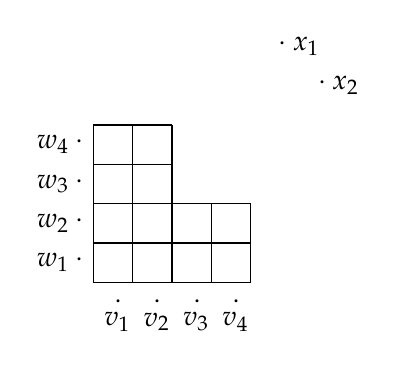
\begin{tikzpicture}[scale=0.5, line width=0.5pt]
  \draw (0,0) grid (4,1);
  \draw (0,0) grid (4,2);
  \draw (0,0) grid (2,3);
  \draw (0,0) grid (2,4);
  
  \node[left] (A) at (1.2,-1) {$v_1$};
  \node[left] (B) at (2.2,-1) {$v_2$};
  \node[left] (C) at (3.2,-1) {$v_3$};
  \node[left] (D) at (4.2,-1) {$v_4$};
  
  \node[left] (A') at (1,-0.5) {$\cdot$};
  \node[left] (B') at (2,-0.5) {$\cdot$};
  \node[left] (C') at (3,-0.5) {$\cdot$};
  \node[left] (D') at (4,-0.5) {$\cdot$};
  
  \node[left] (F) at (0,0.5) {$w_1\:\cdot$};
  \node[left] (G) at (0,1.5) {$w_2\:\cdot$};
  \node[left] (H) at (0,2.5) {$w_3\:\cdot$};
  \node[left] (I) at (0,3.5) {$w_4\:\cdot$};
  
  \node[left] (J) at (6,6) {$\cdot\:x_1$};
  \node[left] (K) at (7,5) {$\cdot\:x_2$};
  
\end{tikzpicture}
  \caption{The staircase graph $G_{10}(\lambda)$ with $\lambda=2\cdot\text{cor}(2)$}
  \label{figure13:Figure 13}
\end{figure}

\end{expl}

The proof of the following statement can be found in \cite{6}.

\begin{thm}
Let \(k+2\) devide \(n\), then we have:
\[
\gamma_k(\Delta^{[n]})=\rho_k(\Delta^{[n]})=\frac{n}{k+2}
\]
\end{thm}

By the previous results we see that the hitting expansion and the disjoint cycle expansion coincide with the Cheeger constant for the simplex in all cases, where we know the Cheeger constant exactly. Up to know we do not know any family of complexes for which these constants differ, but nevertheless we can not show that they coincide in general.
% Chapter 4

\chapter{Perspectives}

\label{Chapter4}

 
% Chapter 4

\chapter{Perspectives}

\label{Chapter4}



%----------------------------------------------------------------------------------------
%	THESIS CONTENT - APPENDICES
%----------------------------------------------------------------------------------------

\appendix % Cue to tell LaTeX that the following "chapters" are Appendices

% Include the appendices of the thesis as separate files from the Appendices folder
% Uncomment the lines as you write the Appendices

\pagenumbering{Roman}

%\chapter{Source code for the Cheeger Tool Box (CTB)}

\label{AppendixA}

The \textit{Cheeger Tool Box (CTB)} is a software library written in C++11, containing methods to handle some important tasks concerning the topic of Cheeger constants of a simplex, such as calculating the cosystolic norm and the coboundary expansion of a given cochain or calculating the \(k\)-th Cheeger constant of a simplex on \(n\) vertices. A cochain \(\varphi\in C^k(\Delta^{[n]})\) is always represented as a column vector with \(\binom{n}{k+1}\) (i.e. a matrix of one column and  \(\binom{n}{k+1}\) lines, such that every entry \(i\) is either \(1\) or \(0\), depending on if the \(i\)-th simplex in the uniform \(k\)-skeleton of \(\Delta^{[n]}\) is contained in the support of \(\varphi\). Here, the simplices of the uniform \(k\)-skeleton of \(\Delta^{[n]}\) are indexed lexicographically based on the contained vertices, which are indexed from \(1\) to \(n\).\\
To use the library, the reader should just save the single files in an ordering as shown in the labellings underneath each code block and include the header files into his own code. Note, that by now the methods only use the basic definitions of cosystolicity and Cheeger constants for the calculation. The interested reader is invited to use more results from theoretical research to improve its performance.\\

\lstinputlisting[language=C++]{CTB/headers/Matrix.h}

\lstinputlisting[language=C++]{CTB/sources/Matrix.cpp}

\lstinputlisting[language=C++]{CTB/headers/basics.h}

\lstinputlisting[language=C++]{CTB/sources/basics.cpp}

\chapter{Source code for 'Partitioning Consecutive Numbers' (PCN)}

\label{AppendixB}

The program \textit{Partitioning Consecutive Numbers (PCN)} realizes the algorithm presented in Chapter \ref{Chapter4} as a console application written in C++11. To use it, the reader should just save the single files in an ordering as shown in the labellings underneath each code block and build all files. Then just type \textit{PCN} followed by three arguments seperated by a space character into the console. The first argument is the number \(n\) representing the sum from \(1\) to \(n\), the second and the third argument are the numbers \(a\) and \(b\) representing the sum from \(a\) to \(b\). Make sure, that the conditions of Theorem \ref{theorem11} are satisfied, meaning \(a\leq b\) and the sum from \(1\) to \(n\) should equal the sum from \(a\) to \(b\). Then the program produces a matrix whose lines respresent the parts of the partition of \([n]\), such that each line sums up to a number between \(a\) and \(b\). The entries of the matrix which are not used become filled with zeros.\\
\\

\lstinputlisting[language=C++]{PCN/sources/PCN.cpp}

\lstinputlisting[language=C++]{PCN/headers/Matrix.h}

\lstinputlisting[language=C++]{PCN/sources/Matrix.cpp}

\lstinputlisting[language=C++]{PCN/headers/basics.h}

\lstinputlisting[language=C++]{PCN/sources/basics.cpp}

\lstinputlisting[language=C++]{PCN/headers/findPartitions.h}

\lstinputlisting[language=C++]{PCN/sources/findPartitions.cpp}

%----------------------------------------------------------------------------------------
%	BIBLIOGRAPHY
%----------------------------------------------------------------------------------------

%\printbibliography[heading=bibintoc]

%----------------------------------------------------------------------------------------
\begin{thebibliography}{1}
\addchaptertocentry{Bibliography}
\bibitem{1}
Dmitry N. Kozlov, \textit{The first Cheeger constant of a simplex}, Graphs and Combinatorics (2017) 33: 1543. https://doi.org/10.1007/s00373-017-1853-9
\bibitem{2}
N. Linial, R. Meshulam, \textit{Homological connectivity of random 2-complexes}, Combinatorica 26, 2006,
no. 4, 475-487
\bibitem{3}
M. Gromov, \textit{Singularities, expanders and topology of maps. Part 2. From combinatorics to topology
via algebraic isoperimetry}, Geom. Funct. Anal. 20, (2010), no. 2, 416-526.
\bibitem{4}
M. Wallach and R. Meshulam, \textit{Homological connectivity of random k-dimensional complexes}, Random Structures Algorithms 34, 2009, no. 3, 408–417
\bibitem{5}
J. J. Sylvester and F. Franklin, \textit{A Constructive Theory of Partitions, Arranged in Three Acts, an Interact and an Exodion}, American Journal of Mathematics
Vol. 5, No. 1 (1882), pp. 251-330
\bibitem{6} Dmitry N. Kozlov and Roy Meshulam, \textit{Quantitative aspects of acyclicity}, arXiv:1802.03210 [math.CO], 2018
\bibitem{7} Peter Keevash, \textit{Hypergraph Tur\'{a}n problems}, Surveys in Combinatorics, Cambridge University Press, 2011
\bibitem{8} Anders Björner and Martin Tancer, \textit{Combinatorial Alexander Duality - A Short and Elementary Proof}, Discrete Comput Geom (2009) 42: 586–593 DOI 10.1007/s00454-008-9102-x, Springer Science+Business Media, LLC 2008
\bibitem{9} Tim Lindemann, \textit{Personal communication}, University of Bremen, 2018
\bibitem{10} Dmitry N. Kozlov, \textit{Personal communication}, University of Bremen, 2017
\bibitem{11} Peter Keevash, \textit{The existence of designs},\\ http://people.maths.ox.ac.uk/keevash/papers/designsI.pdf, 2018
\bibitem{12} Karp R.M., \textit{Reducibility among Combinatorial Problems}. In: Miller R.E., Thatcher J.W., Bohlinger J.D. (eds) Complexity of Computer Computations. The IBM Research Symposia Series. Springer, Boston, MA, 1972
\bibitem{13} Dmitry N. Kozlov, \textit{Personal communication}, University of Bremen, 2019
\end{thebibliography}

\printindex

\end{document}  
